% Options for packages loaded elsewhere
\PassOptionsToPackage{unicode}{hyperref}
\PassOptionsToPackage{hyphens}{url}
%
\documentclass[
]{book}
\usepackage{lmodern}
\usepackage{amssymb,amsmath}
\usepackage{ifxetex,ifluatex}
\ifnum 0\ifxetex 1\fi\ifluatex 1\fi=0 % if pdftex
  \usepackage[T1]{fontenc}
  \usepackage[utf8]{inputenc}
  \usepackage{textcomp} % provide euro and other symbols
\else % if luatex or xetex
  \usepackage{unicode-math}
  \defaultfontfeatures{Scale=MatchLowercase}
  \defaultfontfeatures[\rmfamily]{Ligatures=TeX,Scale=1}
\fi
% Use upquote if available, for straight quotes in verbatim environments
\IfFileExists{upquote.sty}{\usepackage{upquote}}{}
\IfFileExists{microtype.sty}{% use microtype if available
  \usepackage[]{microtype}
  \UseMicrotypeSet[protrusion]{basicmath} % disable protrusion for tt fonts
}{}
\makeatletter
\@ifundefined{KOMAClassName}{% if non-KOMA class
  \IfFileExists{parskip.sty}{%
    \usepackage{parskip}
  }{% else
    \setlength{\parindent}{0pt}
    \setlength{\parskip}{6pt plus 2pt minus 1pt}}
}{% if KOMA class
  \KOMAoptions{parskip=half}}
\makeatother
\usepackage{xcolor}
\IfFileExists{xurl.sty}{\usepackage{xurl}}{} % add URL line breaks if available
\IfFileExists{bookmark.sty}{\usepackage{bookmark}}{\usepackage{hyperref}}
\hypersetup{
  pdftitle={Tools for Working with Data},
  pdfauthor={Nicole Sorhagen, Ph.D.},
  hidelinks,
  pdfcreator={LaTeX via pandoc}}
\urlstyle{same} % disable monospaced font for URLs
\usepackage{color}
\usepackage{fancyvrb}
\newcommand{\VerbBar}{|}
\newcommand{\VERB}{\Verb[commandchars=\\\{\}]}
\DefineVerbatimEnvironment{Highlighting}{Verbatim}{commandchars=\\\{\}}
% Add ',fontsize=\small' for more characters per line
\usepackage{framed}
\definecolor{shadecolor}{RGB}{248,248,248}
\newenvironment{Shaded}{\begin{snugshade}}{\end{snugshade}}
\newcommand{\AlertTok}[1]{\textcolor[rgb]{0.94,0.16,0.16}{#1}}
\newcommand{\AnnotationTok}[1]{\textcolor[rgb]{0.56,0.35,0.01}{\textbf{\textit{#1}}}}
\newcommand{\AttributeTok}[1]{\textcolor[rgb]{0.77,0.63,0.00}{#1}}
\newcommand{\BaseNTok}[1]{\textcolor[rgb]{0.00,0.00,0.81}{#1}}
\newcommand{\BuiltInTok}[1]{#1}
\newcommand{\CharTok}[1]{\textcolor[rgb]{0.31,0.60,0.02}{#1}}
\newcommand{\CommentTok}[1]{\textcolor[rgb]{0.56,0.35,0.01}{\textit{#1}}}
\newcommand{\CommentVarTok}[1]{\textcolor[rgb]{0.56,0.35,0.01}{\textbf{\textit{#1}}}}
\newcommand{\ConstantTok}[1]{\textcolor[rgb]{0.00,0.00,0.00}{#1}}
\newcommand{\ControlFlowTok}[1]{\textcolor[rgb]{0.13,0.29,0.53}{\textbf{#1}}}
\newcommand{\DataTypeTok}[1]{\textcolor[rgb]{0.13,0.29,0.53}{#1}}
\newcommand{\DecValTok}[1]{\textcolor[rgb]{0.00,0.00,0.81}{#1}}
\newcommand{\DocumentationTok}[1]{\textcolor[rgb]{0.56,0.35,0.01}{\textbf{\textit{#1}}}}
\newcommand{\ErrorTok}[1]{\textcolor[rgb]{0.64,0.00,0.00}{\textbf{#1}}}
\newcommand{\ExtensionTok}[1]{#1}
\newcommand{\FloatTok}[1]{\textcolor[rgb]{0.00,0.00,0.81}{#1}}
\newcommand{\FunctionTok}[1]{\textcolor[rgb]{0.00,0.00,0.00}{#1}}
\newcommand{\ImportTok}[1]{#1}
\newcommand{\InformationTok}[1]{\textcolor[rgb]{0.56,0.35,0.01}{\textbf{\textit{#1}}}}
\newcommand{\KeywordTok}[1]{\textcolor[rgb]{0.13,0.29,0.53}{\textbf{#1}}}
\newcommand{\NormalTok}[1]{#1}
\newcommand{\OperatorTok}[1]{\textcolor[rgb]{0.81,0.36,0.00}{\textbf{#1}}}
\newcommand{\OtherTok}[1]{\textcolor[rgb]{0.56,0.35,0.01}{#1}}
\newcommand{\PreprocessorTok}[1]{\textcolor[rgb]{0.56,0.35,0.01}{\textit{#1}}}
\newcommand{\RegionMarkerTok}[1]{#1}
\newcommand{\SpecialCharTok}[1]{\textcolor[rgb]{0.00,0.00,0.00}{#1}}
\newcommand{\SpecialStringTok}[1]{\textcolor[rgb]{0.31,0.60,0.02}{#1}}
\newcommand{\StringTok}[1]{\textcolor[rgb]{0.31,0.60,0.02}{#1}}
\newcommand{\VariableTok}[1]{\textcolor[rgb]{0.00,0.00,0.00}{#1}}
\newcommand{\VerbatimStringTok}[1]{\textcolor[rgb]{0.31,0.60,0.02}{#1}}
\newcommand{\WarningTok}[1]{\textcolor[rgb]{0.56,0.35,0.01}{\textbf{\textit{#1}}}}
\usepackage{longtable,booktabs}
% Correct order of tables after \paragraph or \subparagraph
\usepackage{etoolbox}
\makeatletter
\patchcmd\longtable{\par}{\if@noskipsec\mbox{}\fi\par}{}{}
\makeatother
% Allow footnotes in longtable head/foot
\IfFileExists{footnotehyper.sty}{\usepackage{footnotehyper}}{\usepackage{footnote}}
\makesavenoteenv{longtable}
\usepackage{graphicx,grffile}
\makeatletter
\def\maxwidth{\ifdim\Gin@nat@width>\linewidth\linewidth\else\Gin@nat@width\fi}
\def\maxheight{\ifdim\Gin@nat@height>\textheight\textheight\else\Gin@nat@height\fi}
\makeatother
% Scale images if necessary, so that they will not overflow the page
% margins by default, and it is still possible to overwrite the defaults
% using explicit options in \includegraphics[width, height, ...]{}
\setkeys{Gin}{width=\maxwidth,height=\maxheight,keepaspectratio}
% Set default figure placement to htbp
\makeatletter
\def\fps@figure{htbp}
\makeatother
\setlength{\emergencystretch}{3em} % prevent overfull lines
\providecommand{\tightlist}{%
  \setlength{\itemsep}{0pt}\setlength{\parskip}{0pt}}
\setcounter{secnumdepth}{5}
\usepackage{booktabs}
\usepackage{amsthm}
\makeatletter
\def\thm@space@setup{%
  \thm@preskip=8pt plus 2pt minus 4pt
  \thm@postskip=\thm@preskip
}
\makeatother
\usepackage[]{natbib}
\bibliographystyle{apalike}

\title{Tools for Working with Data}
\author{Nicole Sorhagen, Ph.D.}
\date{2021-01-27}

\begin{document}
\maketitle

{
\setcounter{tocdepth}{1}
\tableofcontents
}
\hypertarget{about-this-book}{%
\chapter{About this book}\label{about-this-book}}

This book describes how to use R as a tool to work with data.

You've mastered research methods, you've studied a psychological phenomenon, you've identified a need for a study, you've planned the study, you've developed and preregistered a hypothesis, you've collected the data -- now what? This guide explains how to use RStudio for data management, data visualization, and data analysis.

RStudio is a free and flexible statistics program. While there are some things in RStudio that can be done with point and click methods, most things are done with commands, or code. The commands use a programming language called R (which is based on another programming language called S). This guide focuses on aspects of R commands that are practical and relevant for a psychology student. While learning a programming language can be intimidating, it is my hope that the small incremental steps that I use in this guide will make the process of learning how to use RStudio similar to learning a statistics program with more point and click options (like JASP and SPSS). In addition to being useful for coursework and research, having a basic understanding of how to use R commands could help you become comfortable learning the basics of other programming languages for things like editing a website.

The flexibility that RStudio provides often results in several ways to complete the same task. Because different options can be useful in different ways, I will often provide more than one way to run an analysis in this guide.

This work is licensed under a Creative Commons Attribution-NoDerivatives 4.0 International License.

\hypertarget{set-up-project-on-rstudio-cloud}{%
\chapter{Set up project on Rstudio Cloud}\label{set-up-project-on-rstudio-cloud}}

We will use Rstudio cloud on this website: \url{https://rstudio.cloud}.

You must first make an Rstudio account by clicking the sign up button in the top right corner. (this is free)

\includegraphics{img/signup.png}

Then join our shared RStudio cloud workspace with the link that I sent you in the email titled `Rstudio cloud shared workspace'.

\textbf{You MUST join our shared workspace.} I will be checking your work through this shared RStudio cloud workspace. Within this shared workspace, I will be able to see everyone's project, but you will only be able to see your project and my project.

Once you are in your Rstudio Cloud account\ldots{}

Expand the R studio cloud options by clicking on the 3 lines in the top left corner.

\includegraphics{img/Picture1.png}

Then select our course (which will be titled the name of course). If you cannot see this option -- then you have not been added to our shared workspace.

Once you are in the Class's shared workspace, open a new project. The new project button is on the top right.

Call this project your last name by clicking on the box that says `Untitled Project' and typing your last name.

\includegraphics{img/Projname.png}

Congrats! You have successfully set up your project on our class RStudio Cloud workplace! You will use this project for all of your R work for the rest of the semester. Next let's learn a bit about the software environment and the R programming language.

\hypertarget{introduction}{%
\chapter{Introduction}\label{introduction}}

This chapter introduces the RStudio cloud environment and describes how to import data into the RStudio cloud.

R cannot handle typos and is case sensitive (`Gender' is not the same as `gender'). If your code will not run check for typos and caps.

Related to this point, do not be afraid to copy and paste with using R. I often copy and paste code and replace variable or dataset names as needed. (This is one of the few times in education where copy and paste is OK!)

\hypertarget{windows-in-rstudio}{%
\section{WINDOWS IN RSTUDIO}\label{windows-in-rstudio}}

RStudio has four panes or windows.

\includegraphics{img/rwindow.png}

\hypertarget{the-source-pane}{%
\subsection{The Source Pane}\label{the-source-pane}}

The source pane has several functions. The most important is that it is where you will write and run R commands. In this book we will use a R script files to do this, which are similar to text files. Another popular file type to write and run R commands in is a R markdown file, which can automatically create reports and manuscripts (see the appendix for more information about R markdown files). The source pane can also display datasets in a spreadsheet like format. The variable names will be listed at the top of each column, followed by the raw data. Multiple files can be opened in the source pane at the same time -- there will be a tab for each opened file at the top of the pane.

\hypertarget{the-console-pane}{%
\subsection{The Console Pane}\label{the-console-pane}}

The console or terminal pane shows a record of the tasks or analyses you have asked RStudio to complete. After you run a command from a R script in the source pane, the execution and output will appear in the console pane.

The \textgreater{} symbol in the last line of the console means that the console is ready for a command. If the \textgreater{} symbol is ever missing, click in the last line of the console and hit the escape button on your keyboard. A \textgreater{} symbol will then appear.

While it is possible to type and run R commands in the console, typing commands in scripts in the source pane is better because the information in the console is not saved when RStudio is closed. When you reopen a project, the console will be reset. So, everything you want to save should be in the script.

\hypertarget{the-environment-and-history-pane}{%
\subsection{The Environment And History Pane}\label{the-environment-and-history-pane}}

The environment pane shows what datasets and objects are currently defined in RStudio's memory. The history tab contains a history of the R commands you've executed. This should be fairly redundant with your R scripts.

\hypertarget{the-filesplotspackageshelp-pane}{%
\subsection{The Files/Plots/Packages/Help Pane}\label{the-filesplotspackageshelp-pane}}

This pane has several purposes. The file tab offers a way to open files in RStudio. The plots tab is where any plots you create will appear. The packages tab is where you can see what packages are currently loaded. You can also install and load packages from here. (Packages will be discussed in more detail in the next section.) Finally, the help tab displays documents to help you use R functions and packages.

\hypertarget{navigating-and-commands}{%
\section{NAVIGATING AND COMMANDS}\label{navigating-and-commands}}

\emph{Use R scripts to type and run commands}

The first step of working in RStudio will always be to open a script.

You can open an existing script by selecting it from the file tab in the files/plots/packages/help pane. R script files end in .R (the intro.R file, descripstats.R, and datavis.R files in the picture below are R script files. They contain the commands for chapters 1 to 3 of this guide. Or you could open an existing script by selecting FILE -\textgreater{} OPEN FILE in the top bar menu and then navigate to the file location.

\includegraphics{img/NAVIGATING AND COMMANDS R15.png}\\
Another option is to open a new script. Do this by selecting from the top bar menu: FILE -\textgreater{} NEW FILE -\textgreater{} R SCRIPT

\includegraphics{img/NAVIGATING AND COMMANDS R16.png}

Another way to open a new script is by clicking on the green circle with a cross in the middle and then selecting R Script.

\includegraphics{img/NAVIGATING AND COMMANDS R17.png}

To save a script, select from the top bar menu: FILE -\textgreater{} SAVE AS.

\emph{R is like a fancy calculator}

In its most basic form, you can think of R as a fancy calculator. For example, type the following equation into the script:

\texttt{2+2}

Then, while the cursor is still in the same line as the equation, click the run button to have R calculate the equation (or run this command).

\includegraphics{img/NAVIGATING AND COMMANDS R18.png}

The command (\texttt{2+2}) and results (\texttt{4}) will appear in the console.

\includegraphics{img/NAVIGATING AND COMMANDS R19.png}

You also could highlight the command you want to execute and then click on the run button. Another way to run a command in a script is by using the command (⌘) and enter keys on a mac (or control + enter on a PC).

\emph{Functions are what makes the calculator fancy.}

In this book we will rarely calculate statistics by entering equations. Instead, we will use functions to tell R to use equations for us. For example, to find the mean of a set a scores (such as 2, 2, and 3) you could use the mean equation:

\texttt{M\ =\ (∑X)/N\ \ =\ =\ \ (2+2+3)/3}

This equation would be entered into R as \texttt{(2+2+3)/3}. After you run this command, the answer (\texttt{2.333333}) would appear in the console. Alternatively, you could use the mean function to tell R that you would like it to calculate the mean of the set of scores. (i.e., \texttt{mean(scores)}).

\emph{Functions act on arguments}

Functions always have parentheses at the end of their names, and inside the parentheses is where you tell R more about what you want it to do. The information inside the parentheses are called arguments. In the same way that verbs act on nouns, functions act on arguments.

\emph{Information is stored in objects}

An object in R stores information. Functions are a kind of object that stores equations or actions. Data are stored in objects called vectors and datasets. The results of an analysis can also be saved as an object, as needed.

Information is assigned to objects with assignment operators. This guide will use the arrow assignment operator (\texttt{\textless{}-}). The equal sign can also be used as an assignment operator. Whatever is on the right of the assignment operator is assigned to whatever is on the left of the operator. For example, the command \texttt{match\ \textless{}-\ read\_csv("matchdata.csv")} assigns the data in the file matchdata.csv to an object called match.

All objects are listed in the environment. The environment can be cleared by clicking on the broom at the top of the environment tab. Or you could use the remove function. For example, \texttt{rm(match)} the object named match will no longer be listed in the environment.

Use the \texttt{\$} symbol to access variables within a dataset object (an object with multiple variables in it). For example, \texttt{match\$age} accesses the variable called age in the dataset object called match. Another way to tell R what data object a variable is in is with a pipe, or \texttt{\%\textgreater{}\%}. Pipes are a way to write strings or series of functions more easily. You can think of it as saying ``then''. For example \texttt{match\ \%\textgreater{}\%\ pull(age)} is telling R to first go to the dataset in the match object then pull the variable called age. In order to use pipes (\texttt{\%\textgreater{}\%}) a package called Tidyverse must be loaded -- we will talk more about packages in the next section.

\emph{R quirks}

Before moving on, we need to talk about a few of R's quirks. First, R is case sensitive. R will treat \texttt{mean} differently than \texttt{Mean}. Because of this some experts suggest always using lowercase letters when naming things. This is something to keep in mind when you are choosing names for the objects that store your data.

Second, R cannot handle typos. If you accidentally typed `men' instead of `mean', R will not know that you really meant mean. The predictive text feature of RStudio can help with this. This means that RStudio will suggest functions and objects as you type.

\includegraphics{img/NAVIGATING AND COMMANDS R110.png}

Finally, R is ambivalent about spaces. R ignores redundant spaces in equations. For example, if you typed \texttt{2\ \ \ \ \ +2} or \texttt{2+2} you would get the same answer as when you typed \texttt{2\ +\ 2}. But there cannot be spaces in object names (this is another thing to keep in mind when naming objects), and there cannot be spaces between a function and its parentheses.

When you get an error message after you run a command, check for capitalization errors, typos, and spacing.

\emph{Trial and error}

In the last sentence I said when you get an error, not if you get an error. This is because errors and having a command not run is inevitable. Errors are just a part of coding. It is even people's jobs to find the errors in professional coder's code.

I often have to play around with a command a bit because it will not run. I like to copy and paste a command and then try something different, so I can see what I already have tried.

So, don't sweat the errors! It happens to everyone!

\emph{Scripts should be a record of your analysis}

While trial and error is expected, it should be clear in a script which commands were eventually used and which were not. This is part of making your scripts useable by others and your future self.

Another way to make scripts shareable is to include notes using the hashtag (\texttt{\#}). R will not treat anything in the same line as a hashtag as a R command.

In the current script we are working on, we could add organization and explanations to our current script by adding \texttt{\#\ R\ is\ like\ a\ calculator} above the equations we have run so far and \texttt{\#\ Packages} to indicate the next section.

\includegraphics{img/NAVIGATING AND COMMANDS R111.png}

Note that the comments appear green in the script.

At the very least, you should include enough comments so that someone else (or even yourself in a few months or so) could read your script and get the basic idea of what you did. Beyond that, the content and degree to which comments are included in scripts is a personal choice. For example, sometimes people note the results of an analyses after its command and others do not. Remember that the information in the console is not saved after RStudio is closed. So, including the results in the script can be useful when you reopen a project.

\hypertarget{packages}{%
\subsection{Packages}\label{packages}}

\textbf{Base R} refers to the functions that automatically come with R. But many people build on top of Base R to make R better. The way they do this is through \textbf{packages}, which contain new R functions. There are thousands of packages that could be added on to base R.

Packages are kind of like apps on your smartphone or computer in several ways. First, there are often several packages that can equally do the same thing. Just like there are several apps that would tell you the weather, there are several packages that would compute descriptive statistics. Moreover, some packages are more well-known and popular than others, just as some apps are really popular and others are not. Like the more popular apps, the well-known packages tend to be well supported, meaning that they are updated, maintained, etc. In this guide I try to focus on the more popular packages.

\textbf{Installing packages}

Another way that packages are like smartphone apps is that they both have to be installed first before they can be used.

In RStudio, packages can be installed through point and click or with a command.

Let's first use the point and click method to install a package called tidyverse. Tidyverse was created by Hadley Wickham and his team with the aim of making various aspects of data analysis in R easier. It is actually a collection of packages, and they include a lot of functions that many people think of as essential for data analysis.

To install a package using the point and click method, select from the top bar menu:

TOOLS -\textgreater{} INSTALL PACKAGES

\includegraphics{img/NAVIGATING AND COMMANDS R112.png}

In the install packages window, type the name of the package you would like to install. For example, type ``tidyverse'' in the packages box. Then click INSTALL.

\includegraphics{img/NAVIGATING AND COMMANDS R113.png}\\
Your screen should look like this when the installation is complete:

\includegraphics{img/NAVIGATING AND COMMANDS R114.png}

Do not proceed until the console says the package has been installed.

Another package we will be using a lot is the psych package. The \textbf{psych} package is a package for personality, psychometric, and psychological research. It has been developed at Northwestern University (maintained by William Revelle) to include useful functions for personality and psychological research.

Let's install this package with the install packages function. The basic setup of this function is:

\texttt{install.packages(“PackageName”)}

\begin{itemize}
\tightlist
\item
  Replace \texttt{PackageName} with the name of the package that you want to install.\\
\item
  Remember the quotation marks here!
\end{itemize}

For example, install the psych package with the following command:

\texttt{install.packages("psych")}

After you type (or copy and paste) this command into a script. Highlight it (or click in the same line as in the command) and then click on the run button (or use the run hot keys).

\includegraphics{img/NAVIGATING AND COMMANDS R115.png}

Again, do not proceed until the console says the package has been installed.

\textbf{Loading packages}

In order to use a package, it must be loaded -- just like in order to use an app on your smartphone, it must be opened. Another analogy is moving information from long term memory to working memory. You will need to load the packages you want to use each time you open RStudio.

In RStudio, packages can be loaded with point and click or with a command.

Let's load tidyverse with the point and click method. To do this, first select the packages tab in the files/plots/packages/help pane.

\includegraphics{img/NAVIGATING AND COMMANDS R116.png}

Then type ``tidyverse'' in the search bar (or scroll through the list). Then check the box next to tidyverse. The loading process will appear in the console immediately.

\includegraphics{img/NAVIGATING AND COMMANDS R117.png}

The output in the console lists the 8 packages that make up Tidyverse (ggplot2, tibble, tidyr, readr, purr, dplyr, stringr, and forcats).

Next let's load the psych package with the library command. The basic set-up of this function is:\\
\texttt{library(PackageName)}

\begin{itemize}
\tightlist
\item
  Replace \texttt{PackageName} with the name of the package.
\end{itemize}

For example, load the psych package with this command:\\
\texttt{library(psych)}

After you run this code in the script, the loading process will appear in the console.

\includegraphics{img/NAVIGATING AND COMMANDS R118.png}

Note that if you had already loaded Tidyverse, there will be a warning message telling you that the alpha function is masked from the ggplot2 package. This means that the psych package and the ggplot2 package both have a function called alpha. This is not a big deal. There is a way to tell R which alpha function you want to use.

In summary, the first time you use a package, you need to install it. Once a package is installed, you will need to tell R that you want to use it by loading it. You only have to install a package in a project once. You will have to load a package every time you open RStudio and want to use it.

\hypertarget{data-things}{%
\section{DATA THINGS}\label{data-things}}

Now that you have a sense of how to navigate and use commands in the RStudio program, let's talk about data -- how to enter it, how to open it, how to set it up correctly, and how to transform it.

\hypertarget{manual-entry}{%
\subsection{Manual Entry}\label{manual-entry}}

Data can be added directly into RStudio. While it is more common to collect data in a spreadsheet or another programs and then open it in RStudio for data analysis, it is still important to review how to enter data directly into RStudio. This section will review how to go about doing this with an example about class tardiness. Let's pretend that someone counted the number of times a week that five students were late for a class that meets on Mondays, Wednesdays, and Fridays. Here is their data:

\includegraphics{img/data.png}

Let's use the concatenate, or combine, function to assign the data to an object. The basic setup of this function looks like this:

\texttt{VariableName\ \textless{}-\ c(X1,\ X2,\ X3,\ etc.)}

\begin{itemize}
\tightlist
\item
  The \texttt{VariableName\ \textless{}-} part of this command saves the data to an object. Replace \texttt{VariableName} with the name of the variable. Variable names should not have spaces or special characters in them. Naming variables is another part of making analyses shareable with others. Variable names should be informative but short (under 15 characters).\\
\item
  The c is the combine (or concatenate) function\\
\item
  In the parenthesis, list the data in a comma separated list.
\end{itemize}

For example, here is the command to create the Student ID column:

\texttt{id\ \textless{}-\ c(1,\ 2,\ 3,\ 4,\ 5)}

\begin{itemize}
\tightlist
\item
  This command is telling R to save an object called studentid that is made up of this list of numbers \texttt{(1,\ 2,\ 3,\ 4,\ 5)}
\end{itemize}

After you run this command, an object called `id' will be listed in the environment pane.

\includegraphics{img/DATA THINGS R11.png}\\
Next let's assign the data for the number of times the students were late in the first week. Let's call this variable latew1 (for late week 1, or the number of times students were late the first week of the study). Here is the command:

\texttt{latew1\ \textless{}-\ c(2,\ 0,\ 1,\ 2,\ 0)}

\begin{itemize}
\tightlist
\item
  This command is telling R to save an object called latew1 that is made up of this list of numbers \texttt{(2,\ 0,\ 1,\ 2,\ 0)}
\end{itemize}

After you run this command, an object called \texttt{latew1} will be listed in the environment pane.

\includegraphics{img/DATA THINGS 1R2.png}

Then enter the week 2 and 3 data with the following commands:

\texttt{latew2\ \textless{}-\ c(3,\ 0,\ 1,\ 2,\ 0)}

\begin{itemize}
\tightlist
\item
  This command is telling R to save an object called latew2 that is made up of this list of numbers (3, 0, 1, 2, 0).
\end{itemize}

\texttt{latew3\ \textless{}-\ c(2,\ 1,\ 0,\ 3,\ 0)}

\begin{itemize}
\tightlist
\item
  This command is telling R to save an object called latew3 that is made up of this list of numbers (2, 1, 0, 3, 0).
\end{itemize}

\includegraphics{img/DATA THINGS 1R3.png}

These variables can be combined into one dataset object with the data.frame function. The basic setup of this function is:

\texttt{DatasetName\ \textless{}-\ data.frame(Variable1,\ Variable2,\ etc)}

\begin{itemize}
\tightlist
\item
  Replace DatasetName with what you want to call you data object. Like the variable names, dataset names should be informative but short (under 15 characters).
\end{itemize}

In the current example the command would look like this:

\texttt{tardy\ \textless{}-\ data.frame(id,\ latew1,\ latew2,\ latew3)}

\begin{itemize}
\tightlist
\item
  This command is saying to assign the data in the id, latew1, latew2, latew3 objects to a dataset object named tardy
\end{itemize}

After you run this command, there will be a new object in the environment called tardy. Note that the tardy object is listed under data and the individual variables are listed under values.

\includegraphics{img/DATA THINGS 1R4.png}

\hypertarget{upload-data-into-rstudio-cloud}{%
\subsection{Upload data into RStudio Cloud}\label{upload-data-into-rstudio-cloud}}

When using RStudio in the cloud, you will first need to upload the data into your project on the website. To do this select the UPLOAD button in the files window.

\includegraphics{img/upload.png}

In the Upload Files window, click the CHOOSE FILE button and then navigate to the file on your computer. Then click the OK button.

\includegraphics{img/choosefile.png}

The data file should now be listed in the files section of RStudio.

\includegraphics{img/filelist.png}

\hypertarget{importing-data-from-other-sources}{%
\subsection{Importing Data From Other Sources}\label{importing-data-from-other-sources}}

Often data is collected in a spreadsheet (like excel or google sheets) or through a survey manager (like Qualtrics or SurveyMonkey) and then is opened into RStudio. Before you can open a data file in RStudio, you need to know the format of the data file. See Table 1.1 for some common file extensions for data.

Let's open the data in the match.csv file (this is the data we will use in the data transformation section of this chapter, as well as in chapters 2 and 3). This data file contains data on 688 people currently on Match.com who were asked to complete a survey about themselves and their relationships. This survey included questions about whether or not they judge other people based on things like their appearance, possessions, etc., as well as demographic information such as highest level of education and age. (We will use this file to explore how judgmental people are on dating sites.)

\begin{itemize}
\tightlist
\item
  The first column contains arbitrary ID numbers to identify the participants\\
\item
  The next column contains the participants' ages
\item
  The third column contains the participants' highest level of education
\item
  The following 12 columns contain the data from the judgement questions (0 = no; 1 = yes)
\item
  The remaining variables are not relevant to the current chapter, so they are not defined here.
\end{itemize}

\emph{note that this data is a subsample of a real data collected through the Kinsey Institute and match.com}

You can open data in RStudio using a point and click method or using a command.

The point and click method of importing data in RStudio is simple and convenient. This method is accessed by clicking on the import dataset button in the environment and history pane.

\includegraphics{img/DATA THINGS 1R5.png}

Select one of the ``from text'' options if the data is formatted in a .csv or .txt file. (I tend to use the readr option here -- but either works fine). Select the ``from excel'' option if the data is in a .xls or .xlsx format. Select the ``from SPSS'' option if the data is in a .sav format. Select the ``from SAS'' option if the data is in a .sasb7dat format. Select the ``from Stata'' option if the data is in a .dta format.

Since the data is in a .csv file, let's select the readr option.

\includegraphics{img/DATA THINGS 1R6.png}

The following window will open:

\includegraphics{img/DATA THINGS 1R7.png}

Click on the BROWSE button. Then navigate to your file.

\includegraphics{img/DATA THINGS 1R8.png}

Inspect the data preview. You should not need to change anything from the default import options.

Before you click import, I suggest you copy the text in the code preview box. After you click import, paste it into your current script. This way you can easily reassign the datafile to an object if needed by running that command.

After you click import, your screen will look like this:

\includegraphics{img/DATA THINGS 1R9.png}

The spreadsheet view of the match dataset will automatically open in the source pane. The variable names are listed at the top of each column, followed by the raw data. Scroll to the right to see all of the data. The object containing the match data will be listed in the environment. We can see that this dataset has 688 observations and 37 variables.

You can close the spreadsheet of the match dataset in the source pane by clicking on the x in the tab. If you would like to see the data again, click on the dataset's object name (in this example match) in the environment tab and the spreadsheet will reopen in the source pane.

You can also open csv data with \texttt{read\_csv} function. The read\_csv function is part of the readr package, which is part of tidyverse. So if tidyverse is loaded, you do not need to load readr. But if it is not, you can load it with this:

\texttt{library(readr)}

The basic set up of the read\_csv function is:

\texttt{DataObject\ \textless{}-\ read\_csv("FileName.csv")}

\begin{itemize}
\tightlist
\item
  This command is telling R to assign the data in a csv file named FileName to an object called DataObject.\\
\item
  Replace DataObject with your preferred name for the object containing the data\\
\item
  Replace FileName with the name of the file your data is in
\end{itemize}

For example, to assign the match data to an object called match, the command would look like this:\\
\texttt{match\ \textless{}-\ read\_csv("matchdata.csv")}

\begin{itemize}
\tightlist
\item
  This command is telling R to assign the data in the matchdata.csv file to an object called match.\\
\item
  Note that this is the same thing as what you copied and pasted during the point and click method.
\end{itemize}

\hypertarget{data-set-up}{%
\subsection{Data Set Up}\label{data-set-up}}

There are several types of data, or scales of measurement, for variables in RStudio. The big ones for us will be: double, which are numbers with decimals, positive/negative, fractions; integer, which are positive whole numbers; character, which are numbers and words, but as text; and factor which are categorical variables, with specific labels.

The glimpse function, which is part of the tidyverse package, gives a nice summary of a dataset including the variable types for all the variables. In order to use this function, the tidyverse package should be loaded (see the loading packages section above).

The basic layout of the glimpse function is:

\texttt{glimpse(DataObject)}

\begin{itemize}
\tightlist
\item
  Replace DataObject with the name of the data object
\end{itemize}

For example, to look at the data types of the variables in the match dataset use this command:

\texttt{glimpse(match)}

After this command is run, the output in the console looks like this:

\includegraphics{img/DATA THINGS R110.png}

The first column lists the names of all of the variables in the dataset. Next, in gray, are the variable types. The dbl stands for double, which is numbers with decimals, positive/negative, fractions. The chr stands for character, or text, data. After the data type, the remainder of the row lists the raw data of the variable.

The data type of a variable can be changed with the \texttt{as.*} function. The * is a placeholder for the different types of data. For example, \texttt{as.factor(VariableName)}, \texttt{as.character(VariableName)}, and \texttt{as.integer(VariableName)}.

\hypertarget{data-transformation}{%
\subsection{Data Transformation}\label{data-transformation}}

Often times there is a need to change data in some way, such as combining variables together to create a summary score. These changes to data are called data transformations. This section covers how to use a RStudio to preform two common types of data transformations: computing a new variable and recoding values.

Let's pretend you were interested in how judgmental people are on dating sites. We can use the match data from the Importing Data section to do this. Remember that the participants completed items about whether or not they judge other people based on certain things. Here are the judgment items:

\includegraphics{img/match.png}
Let's create a total judgment score by summing all of the separate judgment items.

To do this we will use the mutate function. The mutate function is part of the tidyverse package, so you should load tidyverse if you have not done so already (see the loading packages section above).

The basic setup of this function is:

\texttt{mutate(NewVariableName\ =\ New\ variable\ equation)}

\begin{itemize}
\tightlist
\item
  Replace the NewVariableName with the variable name you want. There cannot be spaces or symbols in a variable name. And remember that R is case sensitive, so be mindful of your use of upper and lower case letters. Then list the equation after the equal sign.
\end{itemize}

In addition, you need to tell R which data object to work with. Adding this information makes the command look like this:

\texttt{DataObject\ \%\textgreater{}\%}\\
\texttt{mutate(NewVariableName\ =\ New\ variable\ equation)}

\begin{itemize}
\tightlist
\item
  The \texttt{\%\textgreater{}\%} is called a pipe. Pipes are a way to write strings or series of functions more easily. You can think of it as saying ``then''.\\
\item
  In this example you can read the command as saying ``use the data in the object called DataObject then mutate the variables in that dataset by creating a new variable called NewVariableName which is defined by this equation.\\
\item
  Pipes are part of the tidyverse package.
\end{itemize}

Finally, you need to tell R to save the new variable. Do this with the assignment operator (\texttt{\textless{}-}).

If you want the new variable to be added to a dataset in an existing object, then tell R to reassign the object as itself like this:

\texttt{DataObject\ \textless{}-\ DataObject\ \%\textgreater{}\%}\\
\texttt{mutate(NewVariableName\ =\ New\ variable\ equation)}

Or you could tell R to save the variables in the existing dataset plus the new variable by assigning the work to a new object:

\texttt{NewDataObject\ \textless{}-\ DataObject\ \%\textgreater{}\%}\\
\texttt{mutate(NewVariableName\ =\ New\ variable\ equation)}

\begin{itemize}
\tightlist
\item
  This will save all of the variables in the object named DataObject, plus the variable named NewVariableName into a new object called NewDataObject. After this command is run, NewDataObject will be listed in the environment.
\end{itemize}

For our current example, let's add the total judgment score variable to the match dataset. Here is the command to do so:

\texttt{match\ \textless{}-\ match\ \%\textgreater{}\%}\\
\texttt{mutate(judgmt\ =\ jdgoutfit\ +\ jdgjob\ +\ jdgborn\ +\ jdglive\ +\ jdgcar\ +\ jdguni\ +\ jdgdiet\ +\ jdgdrink\ +\ jdgteeth\ +\ jdgposts\ +\ jdggramr\ +\ jdgsparet)}

\begin{itemize}
\tightlist
\item
  The \texttt{match\ \textless{}-} part of the command tells R to resave the new variable in the object called match.\\
\item
  The \texttt{match\ \%\textgreater{}\%\ mutate} part tells R to use the data in the object called match then mutate\ldots{}\\
\item
  Inside the parenthesis is the new variable, which I called judgmt and its equation, which is the sum of the 12 judgment items.
\end{itemize}

After this command is run, there will be 38 variables in the dataset object called match (remember that originally there were 37).

\includegraphics{img/DATA THINGS R111.png}

If you want, you can see the new variable by opening the dataset (click on the object listed in the environment) and then scroll to the right. The new variable will be in the last column.

\includegraphics{img/DATA THINGS R112.png}

Next let's review how to recode a variable.

Still using the match data, let's pretend you wanted to recode the number of second dates that participants reported having in the last year (This variable is called scnddates). We can see in the codebook that the response options range from 0 to ``over 20''. Let's recode this variable into categories. Let's say that we want to know the number of people that had 0 second dates, and then 1 or 2 second dates, 3 or 4 second dates, and then 5 to 9, 10 to 14, 15 to 19, and 20+.

We can do this with the \texttt{cut} function, which is a pretty cool function of the tidyverse package. Here is the basic command:

\texttt{DataObject\ \textless{}-\ DataObject\ \%\textgreater{}\%}\\
\texttt{mutate(VariableCat\ =\ cut(x\ =\ Variable,}~\\
\texttt{breaks\ =\ c(-Inf,\ N,\ Inf),}~\\
\texttt{labels\ =\ c("-Infinity",\ "N”\ "Infinity")))}

\begin{itemize}
\tightlist
\item
  Replace DataObject with the name of the object containing the data that you are working with.\\
\item
  Replace VariableCat with whatever you want the new variable to be called. I like to use the original variable name followed by ``Cat'' (for categorical).\\
\item
  Replace Variable with the name of the variable you are recoding.\\
\item
  Replace the entries in the breaks parenthesis with where you would like to cut the original variable. First list the lowest value of the first category -- I like to use -Inf (where Inf stands for infinity). Then list the highest value of each category separated by commas (i.e., the second number listed is the highest value of the first category, the third number is the highest value of the second category, and so on). I like to end with Inf, you could also end with the highest value of the last category.\\
\item
  Replace entries in the in labels parenthesis with the corresponding labels that you listed in the breaks.
\end{itemize}

In the match example this command would look like:

\texttt{match\ \textless{}-\ match\ \%\textgreater{}\%}\\
\texttt{mutate(scnddatesCat\ =\ cut(x\ =\ scnddates,}~\\
\texttt{breaks\ =\ c(-Inf,\ 0,\ 2,\ 4,\ 10,\ 15,\ Inf),}~\\
\texttt{labels\ =\ c("0",\ "1\ or\ 2",\ "3\ or\ 4",\ "5\ to\ 9",\ "10\ to\ 15",\ "over\ 15")))}

After this command is run from the script, your screen will look like this:

\includegraphics{img/DATA THINGS R113.png}

There are now 39 variables in the dataset object called match.

Finally, a common type of data transformation in psychology is recoding responses made on a Likert scale. It is common in psychology to have some items of a survey negatively worded and others positively worded. When this happens, we need all of the items to go in the same direction in order to analyze the data. We do this by reverse coding the items going in one direction -- so that a high score on all of the items reflect the same thing.

To reverse code in RStudio, we will use the mutate and recode functions of tidyverse. The basic form of this command is:

\texttt{DataObject\ \textless{}-\ DataObject\ \%\textgreater{}\%}\\
\texttt{mutate(ItemR\ =recode(Item,}OldValue1\texttt{=\ NewValue1,}OldValue2\texttt{=\ NewValue2,\ Etc.)}

\begin{itemize}
\tightlist
\item
  Replace DataObject with the name of the data object\\
\item
  Replace ItemR with whatever you want the new variable to be called. I like to use the original variable name followed by ``R'' (for reverse).\\
\item
  Replace Item with the name of the item that needs to be reverse coded.\\
\item
  Next is a list of the old and new variables. On the left is the old variable and it must be in back ticks (`) when it is a number. String (AKA text) variables should be in quotes ("). On the right is the new value.
\end{itemize}

For example, if responses to the items of a measure were on a 5-point Likert scale and item 2 needed to be reverse coded, the command would look like this:

\texttt{data\ \textless{}-\ data\ \%\textgreater{}\%}\\
\texttt{mutate(item2r\ =recode(item2,}1\texttt{=\ 5,}2\texttt{=\ 4,}3\texttt{=\ 3,}4\texttt{=\ 2,}5\texttt{=\ 1))}

\begin{itemize}
\tightlist
\item
  The data object is called data\\
\item
  item2r will be the name of the new variable.\\
\item
  item2 is the item that is being recoded.\\
\item
  All of the 1's in the data will be recoded as 5's\\
\item
  All of the 2's in the data will be recoded as 4's\\
\item
  All of the 3's will remain 3's\\
\item
  All of the 4's in the data will be recoded as 2's\\
\item
  All of the 5's in the data will be recoded as 1's
\end{itemize}

\hypertarget{picturing-data}{%
\chapter{Picturing Data}\label{picturing-data}}

The first step of data analysis is to look at your data with graphs. Graphs of data are also used to convey the results of a study. In this chapter you will learn how to use RStudio to create frequency distributions, histograms, boxplots, scatterplots, and bar graphs.

\hypertarget{research-question}{%
\section{RESEARCH QUESTION}\label{research-question}}

How often do people judge others? Let's say that we are interested in how judgmental people are on dating sites. Moreover, let's pretend to be interested in whether people's tendencies to judge are related to their age and education.

\hypertarget{method}{%
\section{METHOD}\label{method}}

Pretend that you worked with Dr.~Amanda Gesselman and her colleagues at the Kinsey Institute to create self-report survey items about how often participants judge others. These items were added to a longer semi-proprietary survey about the attitudes and behaviors of single people in the US. This survey was sent to certain people with accounts on match.com. The people were selected so that the demographics match the most recent US census, with oversampling for gay, lesbian, and bisexual participants. Thousands of people completed the survey. We will use a random sample of 688 people from the total sample here.

\hypertarget{data-analysis-overview}{%
\section{DATA ANALYSIS OVERVIEW}\label{data-analysis-overview}}

The data is in file matadatacmplt.csv. This is the same dataset that we used in chapter 1 - except that the total judgement variable is included matadatacmplt and not in the matchdata.csv file. (note that this data is a subsample of real data collected through the Kinsey Institute and Match.com)

• The first column contains arbitrary ID numbers to identify the participants\\
• The next column contains the participants' ages
• The third column contains the participants' highest level of education
• The following 12 columns contain the data from the judgement questions (0 = no; 1 = yes)
• The judgmt column contains the total number of times the participants reported judging others on the 12 items. (this is the variable you made in the data transformation section of chapter 1)
• The remaining variables are not relevant to the current chapter, so they are not defined here. See the codebook (matchcodebook.xlsx) for more information.

After we open the data in RStudio, we will look at it with tables and graphs.

Frequency distributions, histograms and boxplots help you get to know your data and check for errors. Frequency distributions are tables that list all possible values or categories of a variable and their frequency within a study or data set. Histograms are a graph of a frequency table, where all possible values of a variable are on the x-axis and the frequency of each value is on the y-axis.

Boxplots (AKA box and whisker plots) are another way to graphically represent data. The y-axis of a boxplot lists the possible values of a variable. The box represents the Interquartile range (IQR), which is the middle 50\% of scores. The line withing the box shows the median. The highest and lowest scores are represented as whiskers if they are within a certain range (1.5 * IQR). If they are outside of this range, they are represented with a dot because they are considered an outlier. A traditional boxplot can be modified to include dots that represent individual data points (this is becoming increasingly popular because it encourages research transparency). Another popular modification is a violin element, which shows the distribution of the individual data points.

Scatterplots and bar graphs help show your results to others. Scatterplots show the association between two variables. One variable is plotted on the y-axis and the other is plotted on the x-axis. Each dot represents one participant, measured on the two variables. Bar graphs show the association between continuous and categorical variables. They present the means of a continuous variable separately for each level of a categorical variable. Error bars representing the 95\% confidence interval (CI) for each mean should be included in order to represent the variability in the data.

\hypertarget{open-data}{%
\section{OPEN DATA}\label{open-data}}

First assign the dataset to an object called match (or whatever you prefer). You can do this with the point and click method by selecting from the environment menu:

IMPORT DATASET -\textgreater{} FROM TEXT (READR)

\includegraphics{img/2R.1.png}
Click the BROWSE button and then navigate to your file's location on your computer. Then click OPEN and then IMPORT.

Or you could use the following code:

\texttt{match\ \textless{}-\ read\_csv("matchdatacmplt.csv")}

\begin{itemize}
\tightlist
\item
  This command is telling R to assign the data in the matchdatacomplt.csv file to an object called match.
\end{itemize}

Your screen should look like this after the data is imported:

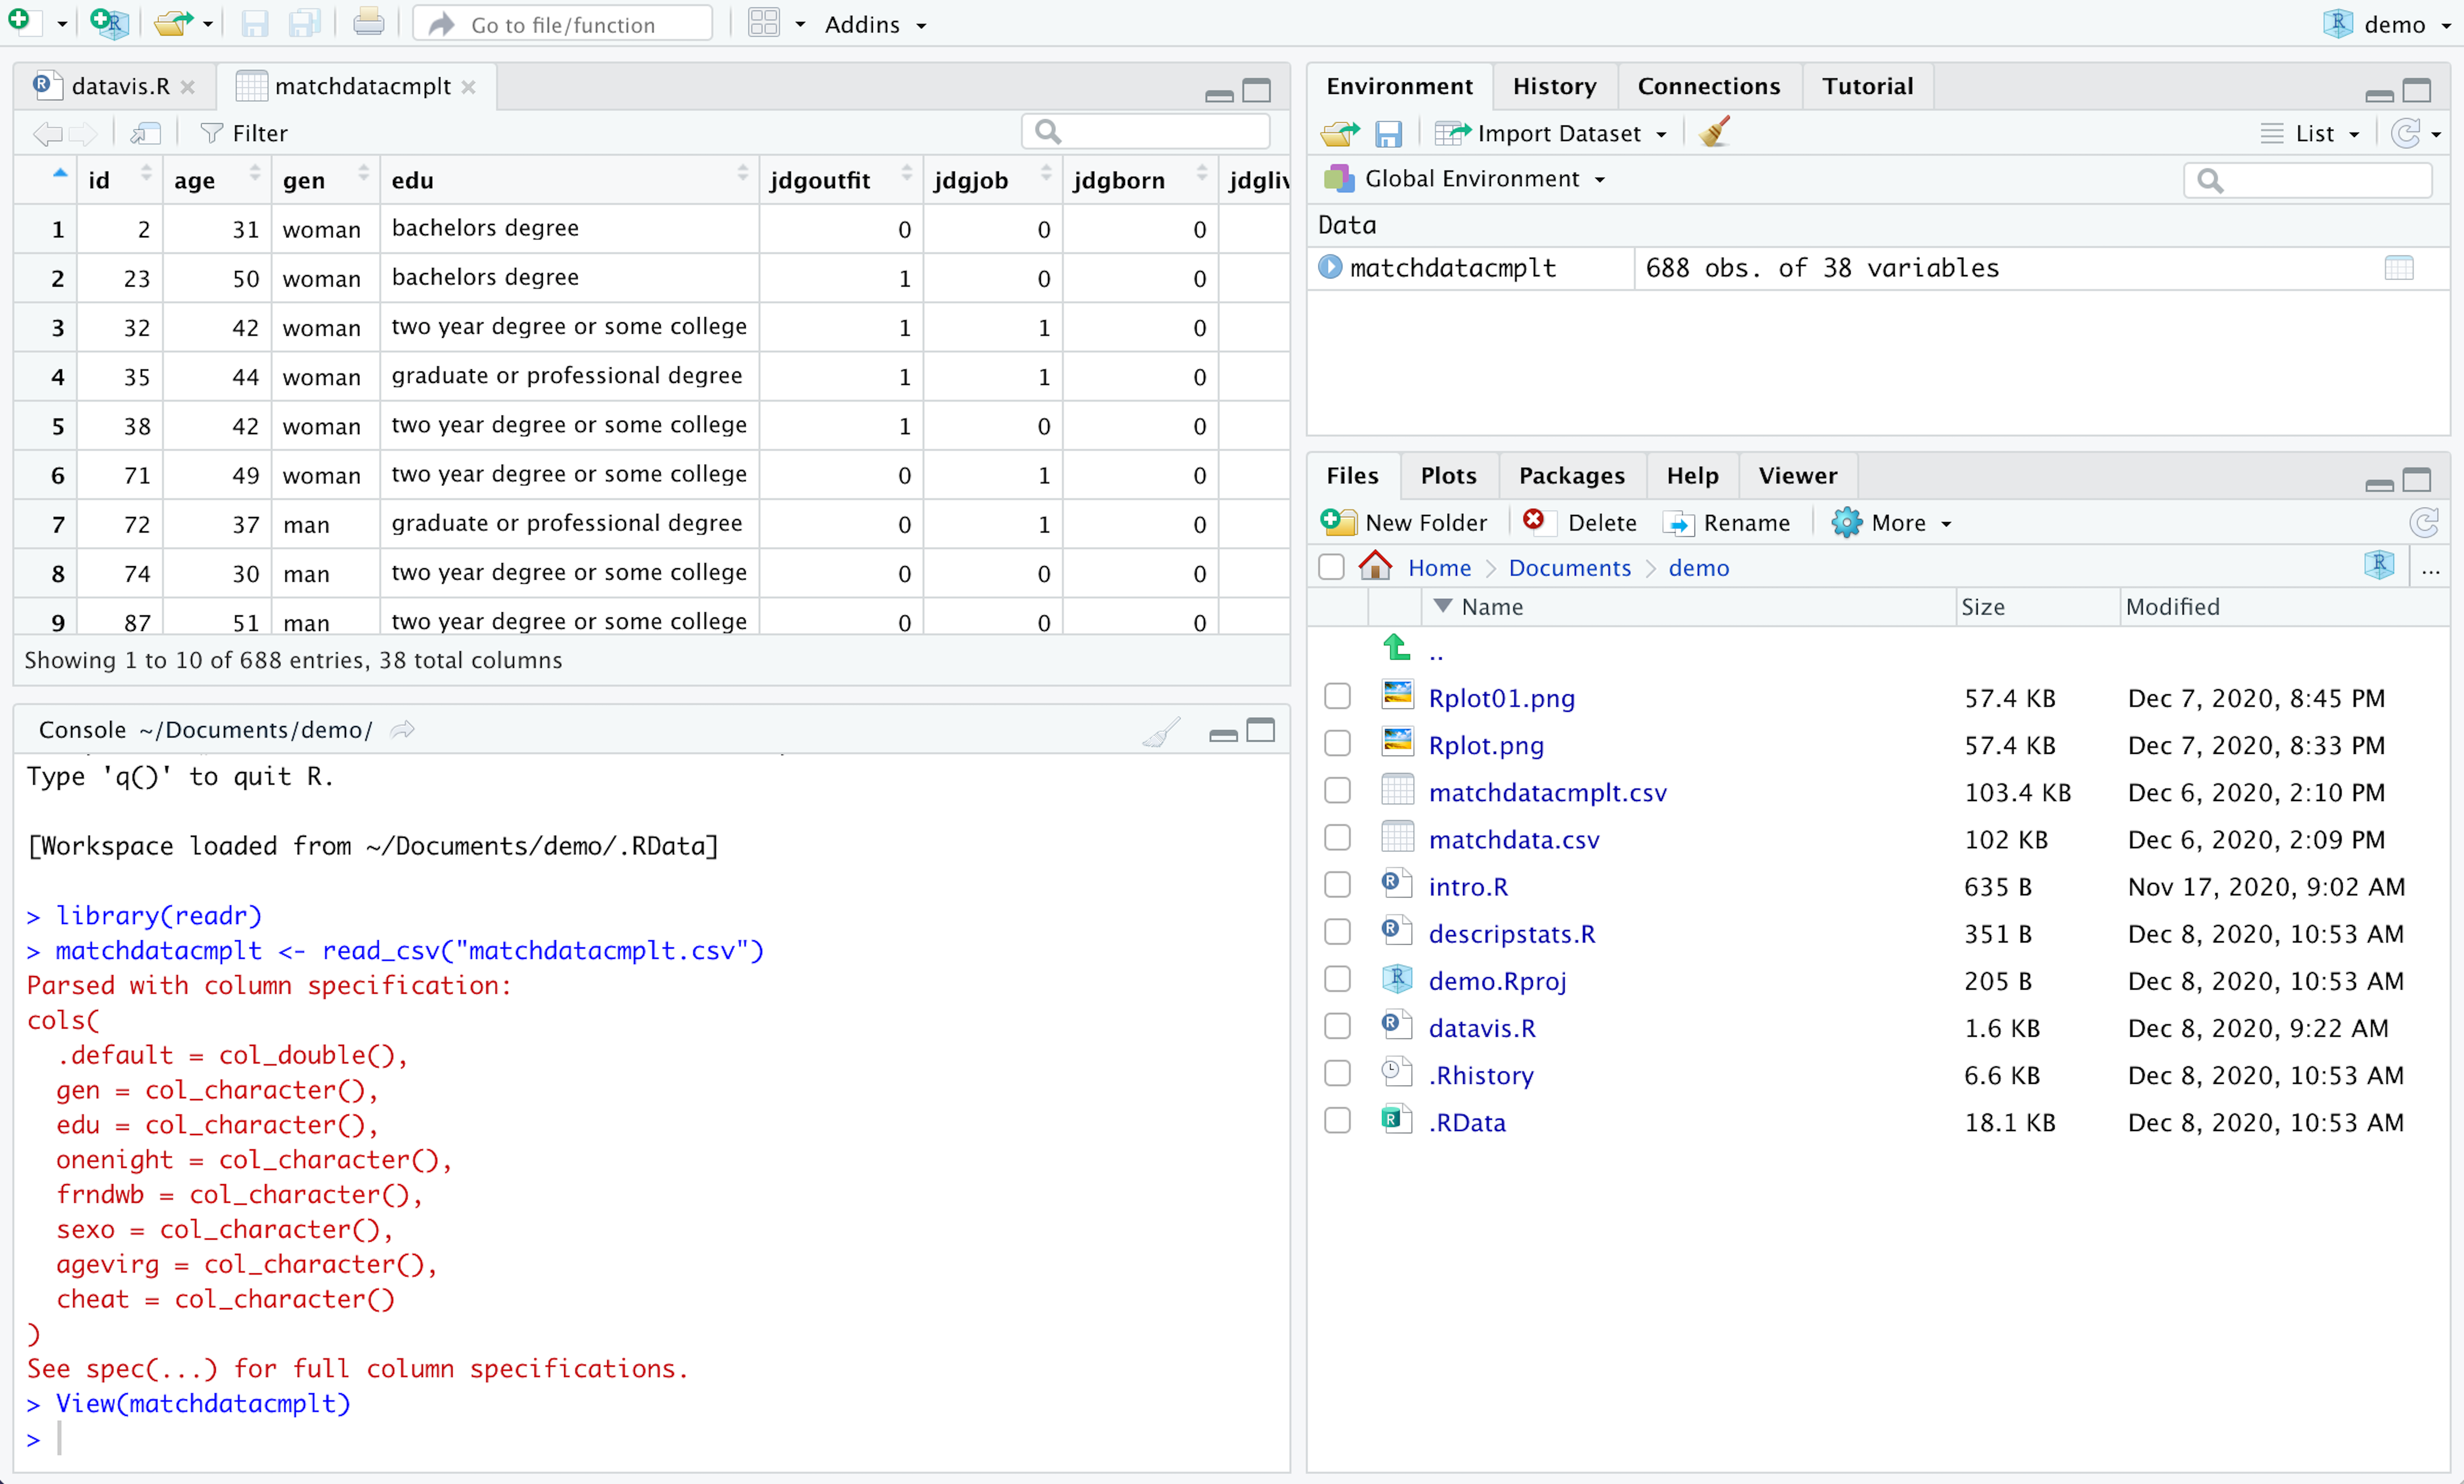
\includegraphics{img/2R.2.png}

\hypertarget{frequency-distribution}{%
\section{FREQUENCY DISTRIBUTION}\label{frequency-distribution}}

Let's first create a frequency distribution of the education variable. One way to do this is with the count function, which is part of the tidyverse package. This function counts the unique values of a variable.

In order to use the count function the tidyverse package must be loaded. If it is not already loaded, load it with this command:

\texttt{library(tidyverse)}\\
(or you could use the point and click method described in chapter 1)

Here is the command to use the count function:

\texttt{DataObject\ \%\textgreater{}\%}\\
\texttt{count(VariableName)}

\begin{itemize}
\tightlist
\item
  This command is saying to first go to the dataset named DataObject and then count all of the unique values of the variable VariableName.
\item
  Replace DataObject with the name of the object that is storing the data.
\item
  Replace VariableName with the name of the variable you would like to count.
\end{itemize}

In this example, use the following command to create a frequency table of the education variable:

\texttt{match\ \%\textgreater{}\%}\\
\texttt{count(edu)}

\begin{itemize}
\tightlist
\item
  This command is telling R to use the data is the match object and count the variable called edu.
\end{itemize}

The frequency table will appear in the console. Your screen should look like this:\\
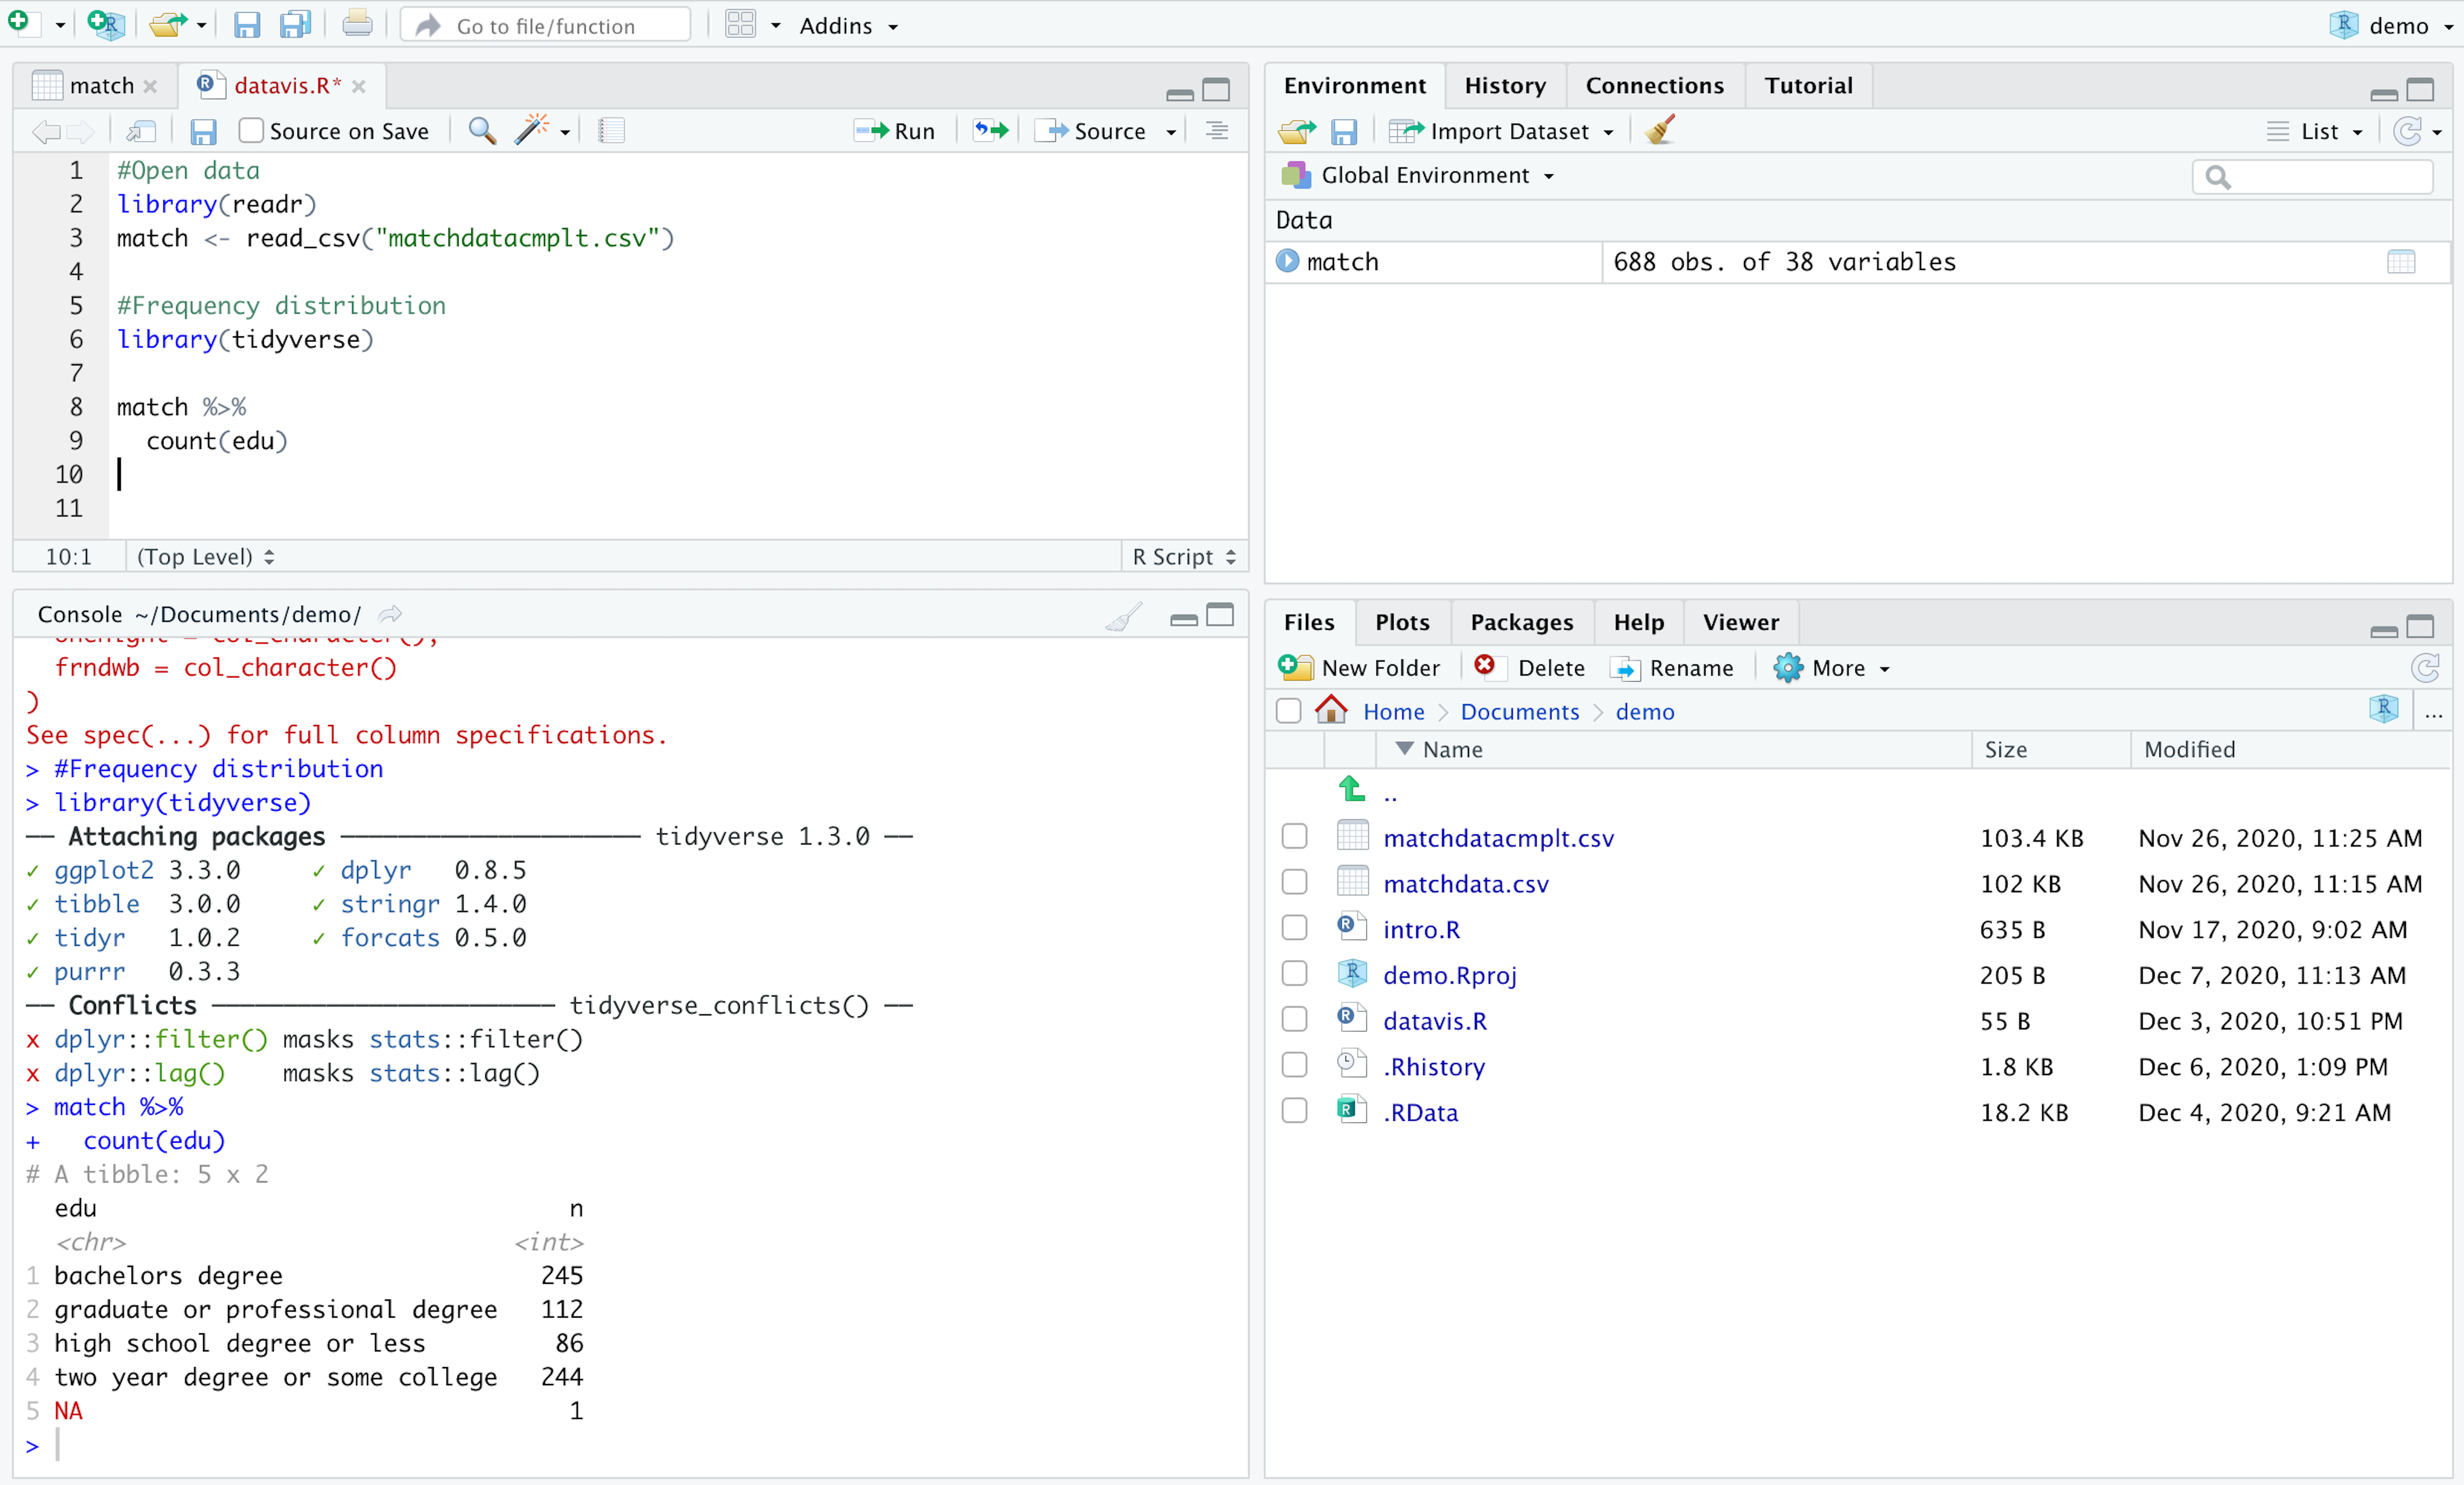
\includegraphics{img/2R.3.png}

The first column of the frequency table lists the levels of the education variable. The NA means not available. This means that this data is missing.

The categories in the frequency table are listed in alphabetical order by default. It is possible to change the order in which RStudio lists the levels of a factor. In the current example it would be nice for the education categories to appear in progressive order. We can do this by using the reorder function, which is part of base R, so no packages need to be loaded in order to use it. Here is what the function looks like in general:

\texttt{DataObject\$VariableName\ \textless{}-\ factor(DataObject\$VariableName,levels\ =\ c("Level1Name",\ "Level2Name",\ "Level3Name",\ "Level4Name"))}

\begin{itemize}
\tightlist
\item
  The \texttt{DataObject\$VariableName\ \textless{}-} saves the reordered levels of the variable called VariableName in the data object called DataObject. Without this the information will not be saved for future use.\\
\item
  The \texttt{factor(DataObject\$VariableName,levels\ =\ c("Level1Name",\ "Level2Name",\ "Level3Name",\ "Level4Name"))} part is what reorders the levels of the factor. The levels should be listed in the new order.\\
\item
  Replace each DataObject with the name of the object that is storing the data.\\
\item
  Replace each VariableName with the name of the variable you would like to count.\\
\item
  Replace the Level1Name with the name of the factor level that you would like to appear first, the Level2Name with the name of the factor level that you would like to appear second, etc.
\end{itemize}

In the current example this looks like this:

\texttt{match\$edu\ \textless{}-\ factor(match\$edu,levels\ =\ c("high\ school\ degree\ or\ less",\ "two\ year\ degree\ or\ some\ college",\ "bachelors\ degree",\ "graduate\ or\ professional\ degree"))}

After you run the reorder command, rerun the count command. The order of the educational attainment categories in the table will now be displayed in sequential order.

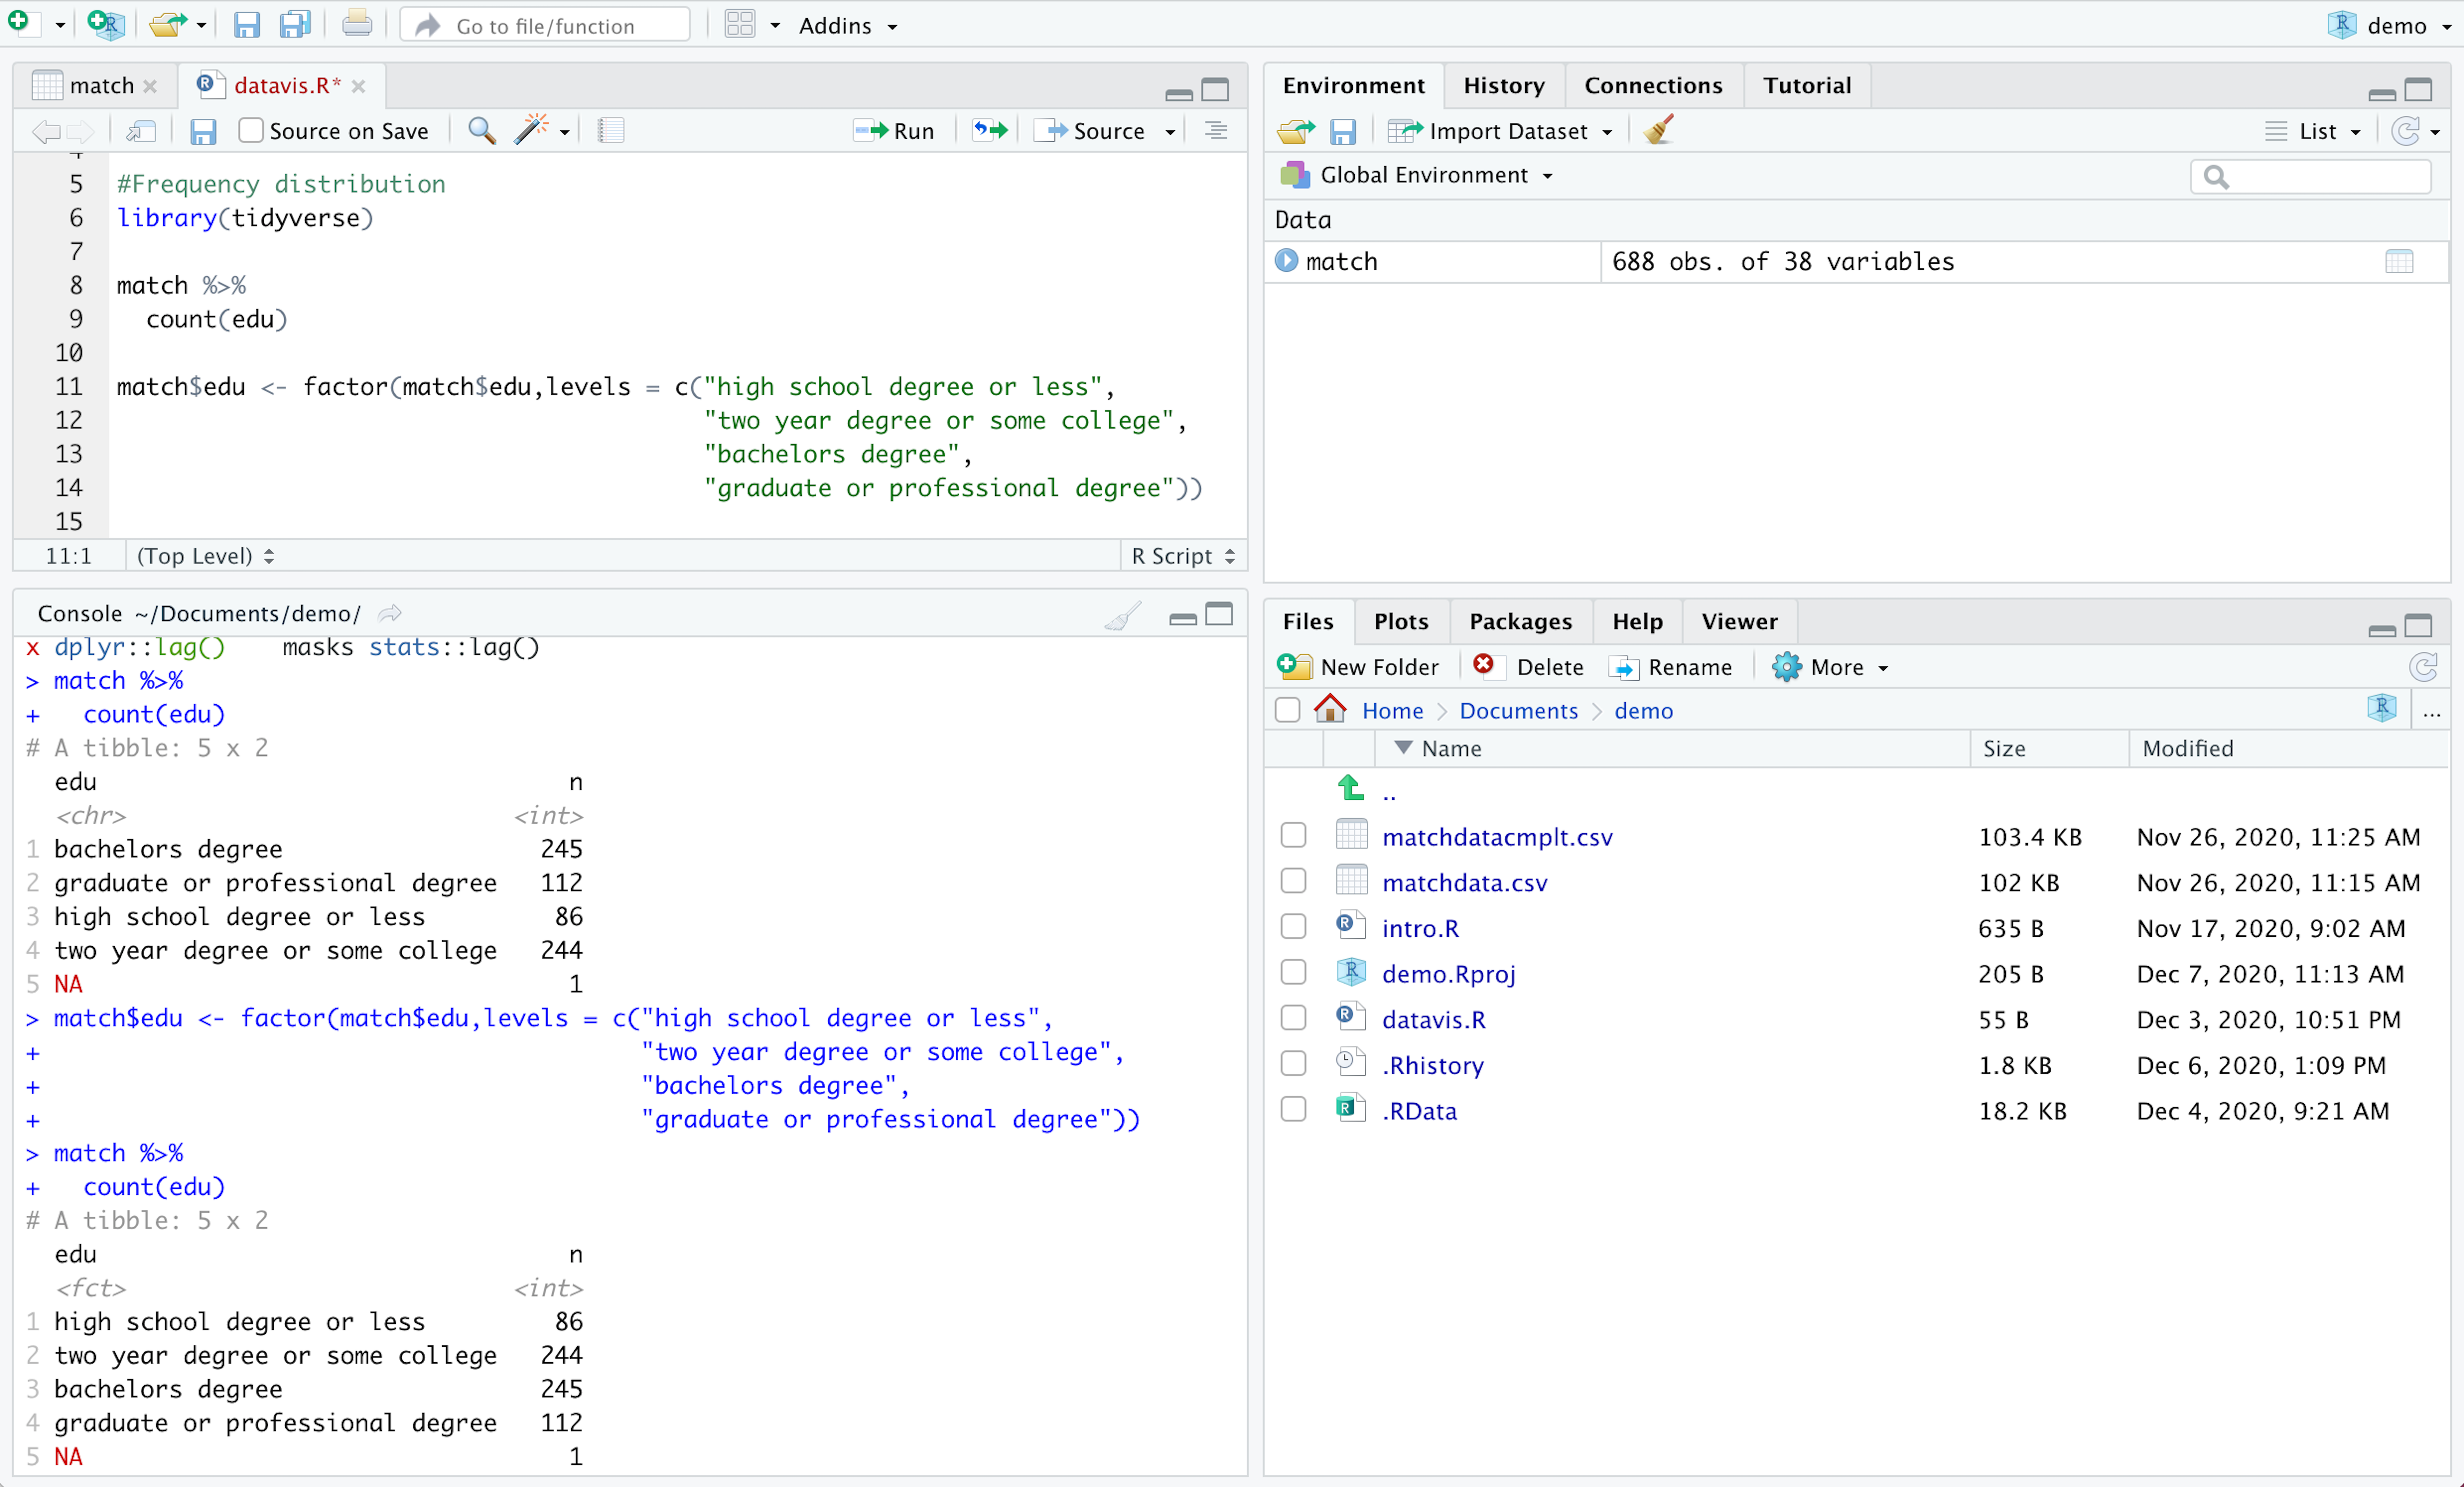
\includegraphics{img/2R.4.png}

The frequency table show that there are 86 people with a high school degree or less; 244 people with an associate, vocational, technical degree or some college, 245 people with a bachelor's degree, and 112 people with a graduate degree. There is missing data for one person. The total sample is 688.

Often, we want to know the percentages of the total sample that the raw frequencies represent. While we could add code to the count function in order to get this information (see appendix for this code), an easier way to get this information is to use a the freq function of the descr package.

In order to use this function the descr package must first be installed. Here is the command to install it:

\texttt{install.packages("descr")}\\
(or you could use the point and click method described in chapter 1)

Once the package is installed, load it with this command:

\texttt{library(descr)}\\
(or you could use the point and click method described in chapter 1)

The freq command looks like this:

\texttt{freq(DataObject\$VariableName)}

\begin{itemize}
\tightlist
\item
  Replace DataObject with the name of the object that is storing the data.\\
\item
  Replace VariableName with the name of the variable you would like to count.
\end{itemize}

In the current example it would look like:\\
\texttt{freq(x\ =\ match\$edu)}

Here is what your screen should look like:

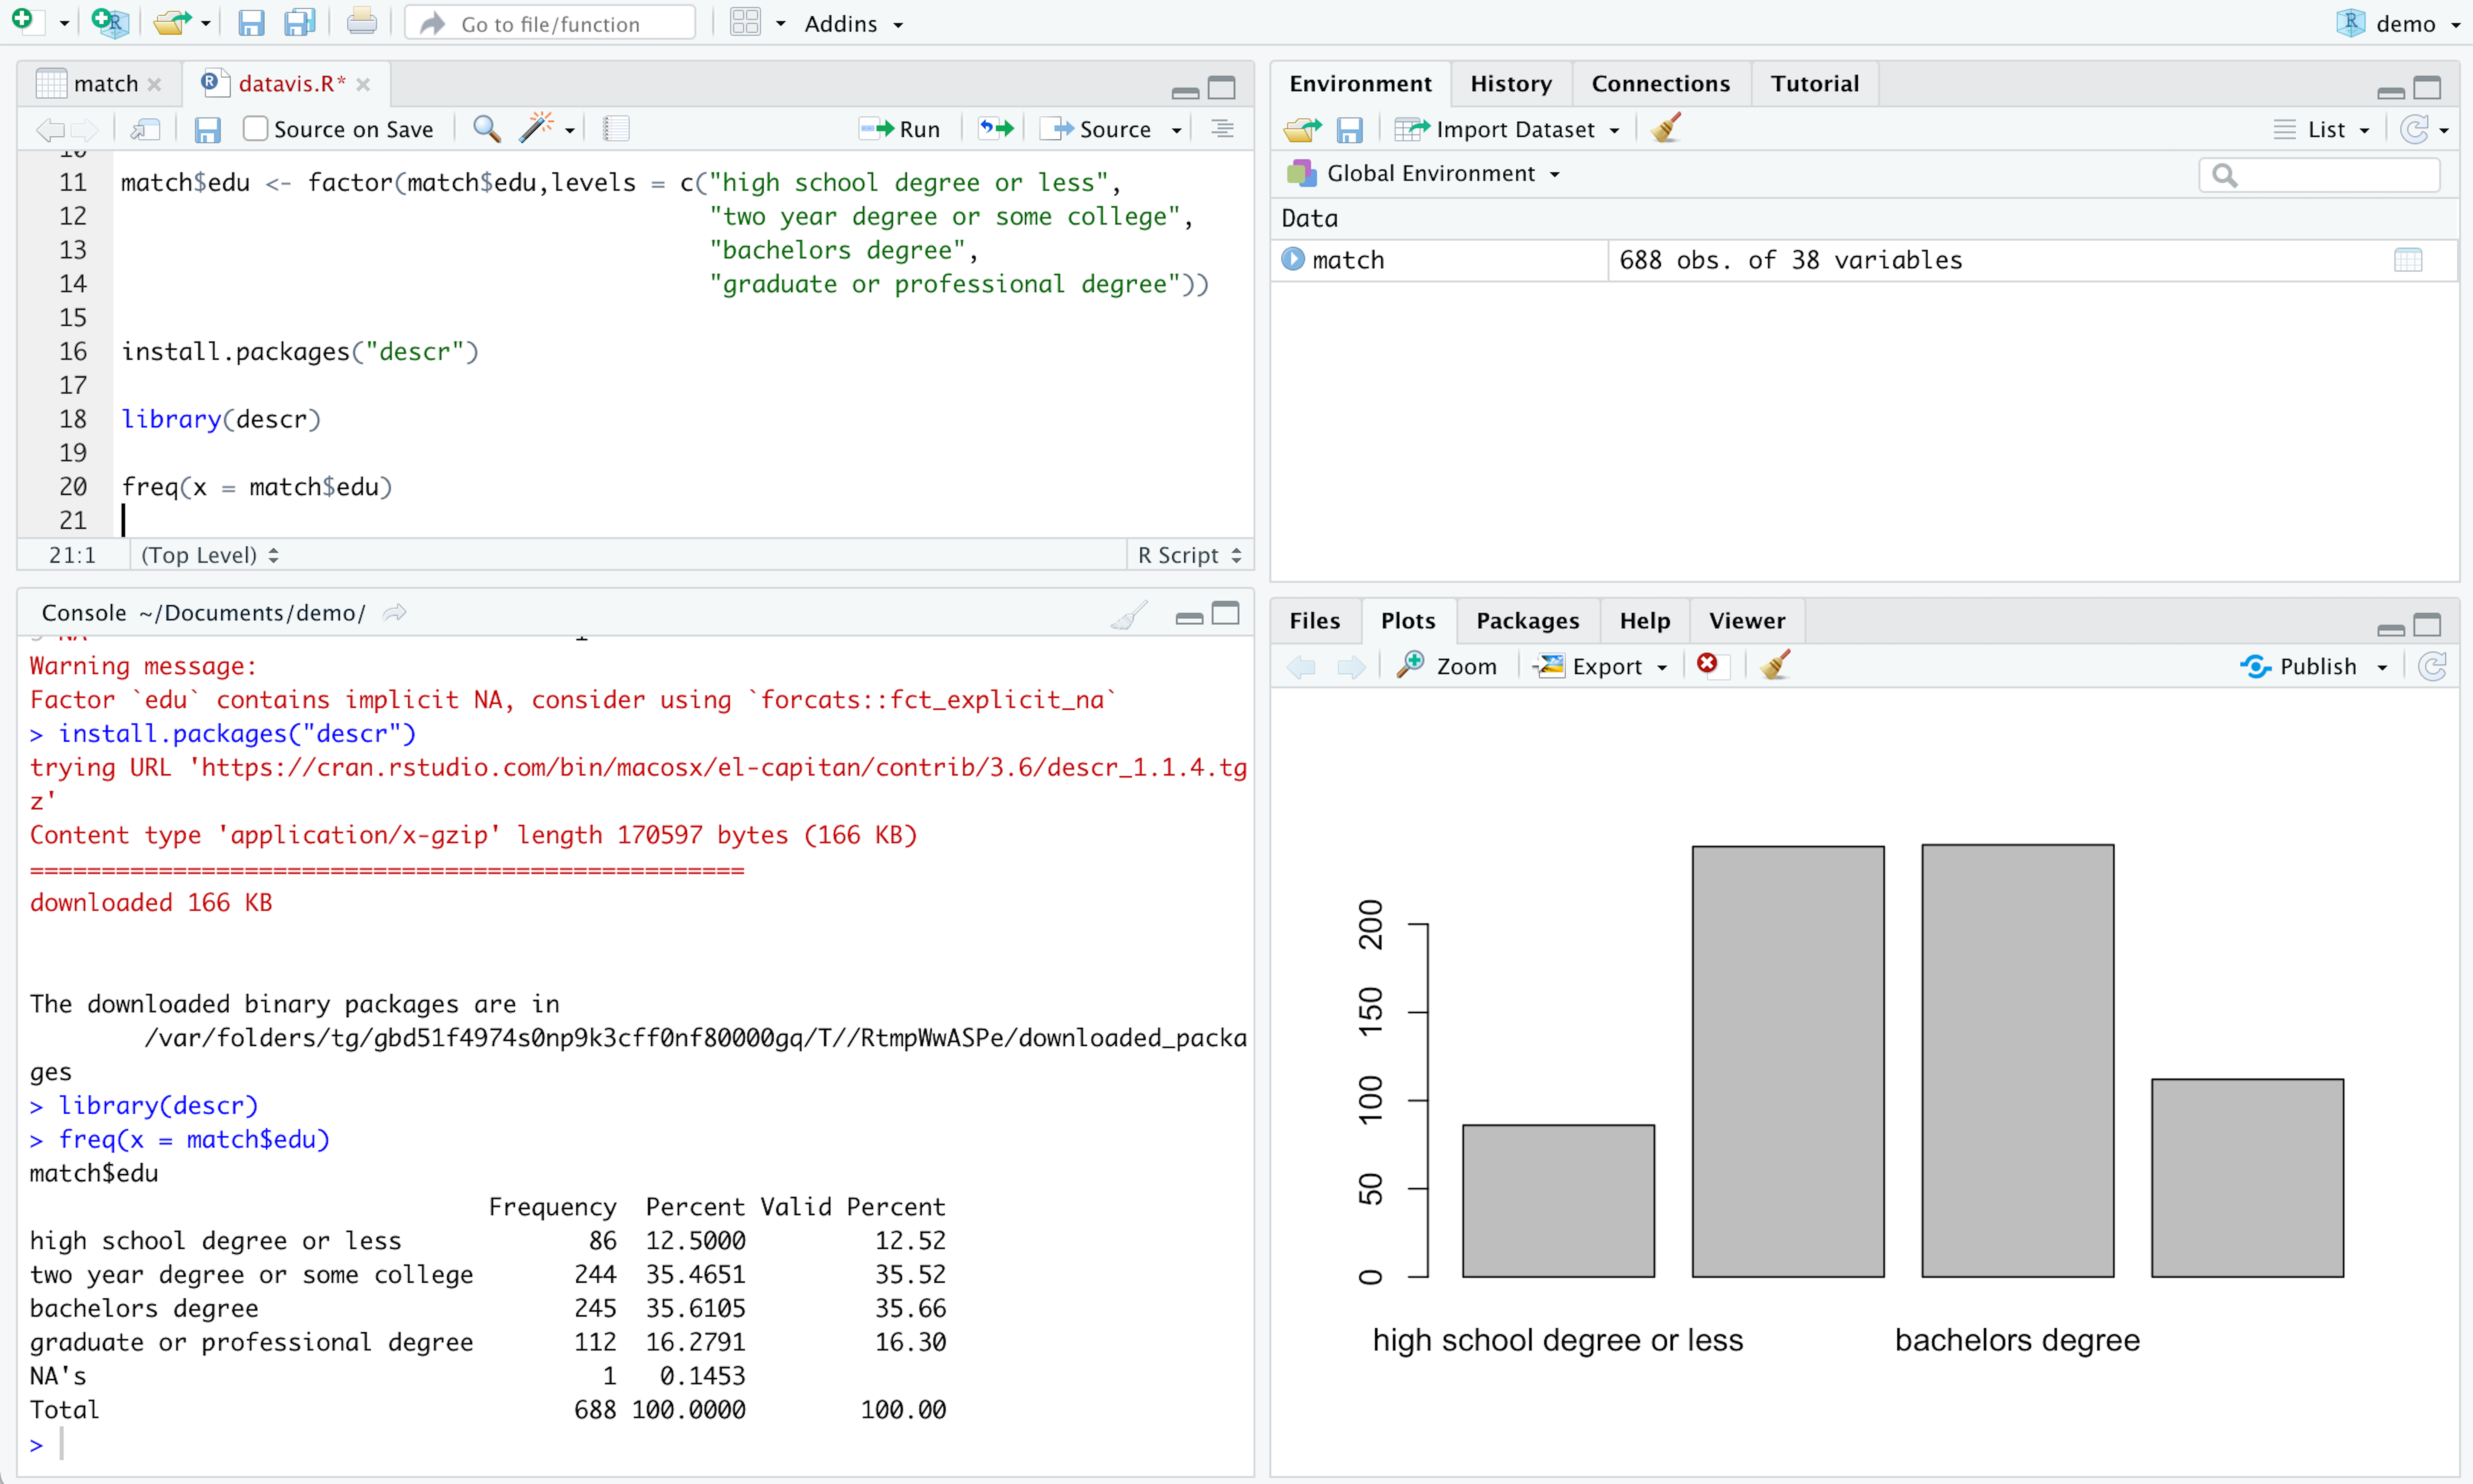
\includegraphics{img/2R.5.png}

Note that the plot on the left-hand side is not very informative. You can suppress this by adding \texttt{plot\ =\ FALSE} in the parenthesis:

\texttt{freq(x\ =\ match\$edu,\ plot\ =\ FALSE)}

The percent column converts the raw frequencies to percentages of the total sample including any missing data. The valid percent column converts the raw frequencies to percentages of the number of non-missing data points. Because there is one data point missing in this example, the percent and valid percent columns are slightly different.

\hypertarget{histograms}{%
\section{HISTOGRAMS}\label{histograms}}

Next let's create a histogram of the age variable. One way to do this is with the hist function, which is part of base R and looks like this:

\texttt{hist(DataObject\$VariableName)}

\begin{itemize}
\tightlist
\item
  Replace DataObject with the name of the object that is storing the data.\\
\item
  Replace VariableName with the name of the variable you would like to plot.
\end{itemize}

Because it is part of base R, no package needs to be loaded in order to use it.

In this example the command to create a histogram of the age variable is:

\texttt{hist(match\$age)}

The plot will appear in the bottom left pane.

\includegraphics{Tools-for-working-with-data-211_files/figure-latex/unnamed-chunk-2-1.pdf}

This histogram provides a more detailed picture of the data because each bar represents the frequency of two years, while the bin width of the histogram that was created with the hist function was 5.

Ggplot is typically taught with the analogy of a globe that is built one layer at a time. It starts with a world of only ocean (no land). Then ``layers'' of land, colors, terrains, legends, etc. are progressively added with additional commands. Use a plus sign (+) to add the layers.

Let's break down the command we used to create the histogram of age to see the step-by-step, layer-by-layer progression of commands that create a ggplot.

First the data set object and the ggplot function creates the blank globe with only ocean:

\includegraphics{img/2R.8.png}

The aesthetic mapping adds the variable data:

\includegraphics{img/2R.9.png}

Then the \texttt{geom\_histogram} adds the graph:

\includegraphics{img/2R.10.png}

Throughout this book we will add on different types of graphs and details to ggplot graphs.

\hypertarget{boxplots}{%
\section{BOXPLOTS}\label{boxplots}}

Let's use a boxplot to look at the data of the judgment variable. This can be done through base R with the boxplot function:

\texttt{boxplot(DataObject\$VariableName)}

\begin{itemize}
\tightlist
\item
  Replace DataObject with the name of the object that is storing the data.\\
\item
  Replace VariableName with the name of the variable you would like to plot.
\end{itemize}

In this example it would look like:

\texttt{boxplot(match\$judgmt)}

After this command is run, the graph will appear in the plots pane:

\includegraphics{img/2R.11.png}

The boxplot shows that most people in our sample are not very judgmental -- 50\% of the data is between 1 and 5 on a 12-point scale. However, the top whisker and outlier point suggest that there are few people in the sample who are very judgmental.

As with the histogram, many people prefer to use ggplot to create a boxplot because it is customizable. The command to do this is:

\texttt{DataObject\ \%\textgreater{}\%}\\
\texttt{ggplot(aes(x\ =\ "",\ y\ =\ VariableName))\ +}~\\
\texttt{geom\_boxplot()}

\begin{itemize}
\tightlist
\item
  Replace DataObject with the name of the object that is storing the data.\\
\item
  Replace VariableName with the name of the variable you would like to plot.\\
\item
  The ""is a placeholder because we want the frequency of Y (rather than adding a second variable).
\end{itemize}

In the current example the command looks and resulting graph likes this:

\begin{Shaded}
\begin{Highlighting}[]
\NormalTok{match }\OperatorTok\StringTok{ }
\StringTok{  }\KeywordTok{ggplot}\NormalTok{(}\KeywordTok{aes}\NormalTok{(}\DataTypeTok{x =} \StringTok{""}\NormalTok{, }\DataTypeTok{y =}\NormalTok{ judgmt)) }\OperatorTok{+}
\StringTok{  }\KeywordTok{geom_boxplot}\NormalTok{()}
\end{Highlighting}
\end{Shaded}

\includegraphics{Tools-for-working-with-data-211_files/figure-latex/unnamed-chunk-3-1.pdf}

This looks very similar to the base R boxplot. However, unlike in base r, additional elements and details can be added to the boxplot when using ggplot. For example, individual data points can be added to a boxplot with the geom\_point option:

\texttt{DataObject\ \%\textgreater{}\%}\\
\texttt{ggplot(aes(x\ =\ "",\ y\ =\ VariableName))\ +}~\\
\texttt{geom\_boxplot()\ +}~\\
\texttt{geom\_point()}

\begin{itemize}
\tightlist
\item
  Replace DataObject with the name of the object that is storing the data.
\item
  Replace VariableName with the name of the variable you would like to plot.
\item
  The geom\_point()tells R to add the raw data to the boxplot. Add \texttt{position\ =\ "jitter",\ color\ =\ "grey"\ in\ the\ geom\_point\ parentheses(i.e.,\ geom\_point(position\ =\ "jitter",\ color\ =\ "grey")} if there are a lot of participants in the dataset because it helps with readability. It is telling R to jitter, or to add random noise to the data points. Without it the data points would overlap each other. The color adds color to an object. I picked grey here, but you can pick any color (yellow, blue, etc.). The point of the color is to make it easier to tell the difference between the data and the rest of the graph.
\end{itemize}

Because the N for the match data set is on the larger side, we should add the jitter and color to the data points.

Here is what the command and graph look like for the current example:

\begin{Shaded}
\begin{Highlighting}[]
\NormalTok{match }\OperatorTok\StringTok{ }
\StringTok{  }\KeywordTok{ggplot}\NormalTok{(}\KeywordTok{aes}\NormalTok{(}\DataTypeTok{x =} \StringTok{""}\NormalTok{, }\DataTypeTok{y =}\NormalTok{ judgmt)) }\OperatorTok{+}
\StringTok{  }\KeywordTok{geom_boxplot}\NormalTok{() }\OperatorTok{+}
\StringTok{  }\KeywordTok{geom_point}\NormalTok{(}\DataTypeTok{position =} \StringTok{"jitter"}\NormalTok{, }\DataTypeTok{color =} \StringTok{"grey"}\NormalTok{)}
\end{Highlighting}
\end{Shaded}

\includegraphics{Tools-for-working-with-data-211_files/figure-latex/unnamed-chunk-4-1.pdf}

This graph shows us that there are more data points at the bottom of the judgmental distribution (less judgmental) than the top.

Instead of the individual data points, the distribution of data points can be added to a boxplot with the geom\_violin option like this:

\texttt{DataObject\ \%\textgreater{}\%}\\
\texttt{ggplot(aes(x\ =\ "",\ y\ =\ VariableName))\ +}~\\
\texttt{geom\_boxplot()\ +}~\\
\texttt{geom\_violin(alpha\ =\ .5)}

\begin{itemize}
\tightlist
\item
  Replace DataObject with the name of the object that is storing the data.\\
\item
  Replace VariableName with the name of the variable you would like to plot.\\
\item
  The alpha = . 5 tells R to make the violin distribution transparent so that the boxplot is still visible. The alpha makes objects transparent. I pick .50, which is half transparent, .75 would be darker and .25 would be lighter.
\end{itemize}

Which looks like this in the current example:

\begin{Shaded}
\begin{Highlighting}[]
\NormalTok{match }\OperatorTok\StringTok{ }
\StringTok{  }\KeywordTok{ggplot}\NormalTok{(}\KeywordTok{aes}\NormalTok{(}\DataTypeTok{x =} \StringTok{""}\NormalTok{, }\DataTypeTok{y =}\NormalTok{ judgmt)) }\OperatorTok{+}
\StringTok{  }\KeywordTok{geom_boxplot}\NormalTok{() }\OperatorTok{+}\StringTok{   }
\StringTok{  }\KeywordTok{geom_violin}\NormalTok{(}\DataTypeTok{alpha =} \FloatTok{.5}\NormalTok{)}
\end{Highlighting}
\end{Shaded}

\includegraphics{Tools-for-working-with-data-211_files/figure-latex/unnamed-chunk-5-1.pdf}

In this example, the violin plot does a better job at showing that there are more people at the lower end of the distribution of judgmental scores.

\hypertarget{scatterplots}{%
\section{SCATTERPLOTS}\label{scatterplots}}

Next let's create a scatterplot between the judgement and age variables. One way to do this is with the plot function of base R, which looks like this:

\texttt{plot(DataObject\$Variable1Name,\ DataObject\$Variable2Name)}

\begin{itemize}
\tightlist
\item
  Replace DataObject with the name of the object that is storing the data.\\
\item
  Replace Variable1Name with the name of one of the variables and Variable2Name with the other.
\end{itemize}

In the current example, the plot function would look like this:

\begin{Shaded}
\begin{Highlighting}[]
\KeywordTok{plot}\NormalTok{(match}\OperatorTok{$}\NormalTok{judgmt, match}\OperatorTok{$}\NormalTok{age)}
\end{Highlighting}
\end{Shaded}

\includegraphics{Tools-for-working-with-data-211_files/figure-latex/unnamed-chunk-6-1.pdf}

The ggplot command for a scatterplot is:

\texttt{DataObject\ \%\textgreater{}\%}\\
\texttt{ggplot(aes(x\ =\ Variable1Name,\ y\ =\ Variable2Name))\ +}~\\
\texttt{geom\_point()}

\begin{itemize}
\tightlist
\item
  Replace DataObject with the name of the object that is storing the data.\\
\item
  Replace Variable1Name with the name of one of the variables and Variable2Name with the other.
\end{itemize}

In the current example this would look like this:

\begin{Shaded}
\begin{Highlighting}[]
\NormalTok{match }\OperatorTok\StringTok{ }
\StringTok{  }\KeywordTok{ggplot}\NormalTok{(}\KeywordTok{aes}\NormalTok{(}\DataTypeTok{x =}\NormalTok{ age, }\DataTypeTok{y =}\NormalTok{ judgmt)) }\OperatorTok{+}
\StringTok{  }\KeywordTok{geom_point}\NormalTok{()}
\end{Highlighting}
\end{Shaded}

\includegraphics{Tools-for-working-with-data-211_files/figure-latex/unnamed-chunk-7-1.pdf}

Here you can see a slight negative trend, such that the younger people in the sample have slightly higher judgmental scores than the older people in the sample (the correlation coefficient (r) = -.15).

\hypertarget{bar-graph}{%
\section{BAR GRAPH}\label{bar-graph}}

Finally, let's make a bar graph of an association between a categorical and continuous variable. For this example, let's look at the association between education and how many times participants reported judging others. To do this we will make a graph of the mean judgment score for each level of education.

Since we are plotting a summary statistic (a mean) instead of raw data (as we did with the histogram and scatterplot), we have to set up our ggplot command a little differently. After specifying the data object and aesthetic, we will use the stat\_summary function to tell R that we want to plot the means with a bar graph. Here is what this looks like:

\texttt{DataObject\ \%\textgreater{}\%}\\
\texttt{ggplot(aes(x\ =\ Variable1Name,\ y\ =\ Variable2Name))\ +}~\\
\texttt{stat\_summary(fun\ =\ mean,\ geom\ =\ "bar")}

\begin{itemize}
\tightlist
\item
  Replace DataObject with the name of the object that is storing the data.
\item
  Replace Variable1Name with the name of the categorical variable and Variable2Name with the name of the continuous variable.
\end{itemize}

Here is the command and graph for the current example:

\begin{Shaded}
\begin{Highlighting}[]
\NormalTok{ match }\OperatorTok\StringTok{ }
\StringTok{  }\KeywordTok{ggplot}\NormalTok{(}\KeywordTok{aes}\NormalTok{(}\DataTypeTok{x =}\NormalTok{ edu, }\DataTypeTok{y =}\NormalTok{ judgmt)) }\OperatorTok{+}
\StringTok{  }\KeywordTok{stat_summary}\NormalTok{(}\DataTypeTok{fun =}\NormalTok{ mean, }\DataTypeTok{geom =} \StringTok{"bar"}\NormalTok{) }
\end{Highlighting}
\end{Shaded}

\includegraphics{Tools-for-working-with-data-211_files/figure-latex/unnamed-chunk-8-1.pdf}

The graph includes the mean for the one person who did not complete the education question of the survey. The NA category can be dropped by adding the drop.na function to the ggplot plot by adding \texttt{drop\_na(Variable1Name)\ \%\textgreater{}\%}. In the current example this looks like:

\begin{Shaded}
\begin{Highlighting}[]
\NormalTok{match }\OperatorTok\StringTok{ }
\StringTok{  }\KeywordTok{drop_na}\NormalTok{(edu) }\OperatorTok
\StringTok{  }\KeywordTok{ggplot}\NormalTok{(}\KeywordTok{aes}\NormalTok{(}\DataTypeTok{x =}\NormalTok{ edu, }\DataTypeTok{y =}\NormalTok{ judgmt)) }\OperatorTok{+}
\StringTok{  }\KeywordTok{stat_summary}\NormalTok{(}\DataTypeTok{fun =}\NormalTok{ mean, }\DataTypeTok{geom =} \StringTok{"bar"}\NormalTok{)}
\end{Highlighting}
\end{Shaded}

\includegraphics{Tools-for-working-with-data-211_files/figure-latex/unnamed-chunk-9-1.pdf}

Finally, 95\% confidence intervals around each mean should be added. Use another stat\_summary function to tell R that you would like to plot the standard of the mean with error bars by adding this line \texttt{stat\_summary(fun.data\ =\ mean\_se,\ geom\ =\ "errorbar",\ width\ =\ .3)}. In the current example this looks like:

\begin{Shaded}
\begin{Highlighting}[]
\NormalTok{match }\OperatorTok\StringTok{ }
\StringTok{  }\KeywordTok{drop_na}\NormalTok{(edu) }\OperatorTok
\StringTok{  }\KeywordTok{ggplot}\NormalTok{(}\KeywordTok{aes}\NormalTok{(}\DataTypeTok{x =}\NormalTok{ edu, }\DataTypeTok{y =}\NormalTok{ judgmt)) }\OperatorTok{+}
\StringTok{  }\KeywordTok{stat_summary}\NormalTok{(}\DataTypeTok{fun =}\NormalTok{ mean, }\DataTypeTok{geom =} \StringTok{"bar"}\NormalTok{) }\OperatorTok{+}\StringTok{ }
\StringTok{  }\KeywordTok{stat_summary}\NormalTok{(}\DataTypeTok{fun.data =}\NormalTok{ mean_se, }\DataTypeTok{geom =} \StringTok{"errorbar"}\NormalTok{, }\DataTypeTok{width =} \FloatTok{.3}\NormalTok{) }
\end{Highlighting}
\end{Shaded}

\includegraphics{Tools-for-working-with-data-211_files/figure-latex/unnamed-chunk-10-1.pdf}

Finally, if you would like to present this graph professionally, the additional options can be added to the ggplot command to adjust color and labels. The theme\_classic function will change the background to white, remove gridlines and add x and y axis lines. The xlab and ylab function will add labs to the respective axis.

\begin{Shaded}
\begin{Highlighting}[]
\NormalTok{match }\OperatorTok\StringTok{ }
\StringTok{  }\KeywordTok{drop_na}\NormalTok{(edu) }\OperatorTok
\StringTok{  }\KeywordTok{ggplot}\NormalTok{(}\KeywordTok{aes}\NormalTok{(}\DataTypeTok{x =}\NormalTok{ edu, }\DataTypeTok{y =}\NormalTok{ judgmt)) }\OperatorTok{+}
\StringTok{  }\KeywordTok{stat_summary}\NormalTok{(}\DataTypeTok{fun =}\NormalTok{ mean, }\DataTypeTok{geom =} \StringTok{"bar"}\NormalTok{) }\OperatorTok{+}\StringTok{ }
\StringTok{  }\KeywordTok{stat_summary}\NormalTok{(}\DataTypeTok{fun.data =}\NormalTok{ mean_se, }\DataTypeTok{geom =} \StringTok{"errorbar"}\NormalTok{, }\DataTypeTok{width =} \FloatTok{.3}\NormalTok{) }\OperatorTok{+}
\StringTok{  }\KeywordTok{theme_classic}\NormalTok{() }\OperatorTok{+}
\StringTok{  }\KeywordTok{xlab}\NormalTok{(}\StringTok{"Education"}\NormalTok{) }\OperatorTok{+}\StringTok{ }\KeywordTok{ylab}\NormalTok{(}\StringTok{"Mean Judgement Score"}\NormalTok{)}
\end{Highlighting}
\end{Shaded}

\includegraphics{Tools-for-working-with-data-211_files/figure-latex/unnamed-chunk-11-1.pdf}

This graph shows that the mean judgmental score increases with educational attainment.

  \bibliography{book.bib,packages.bib}

\end{document}
